\documentclass[lualatex,professionalfonts,aspectratio=169,usepdftitle=false,xcolor={dvipsnames}]{beamer}

\usepackage[utf8]{inputenc}
\usepackage{fontspec}
\usepackage{unicode-math}

\usepackage[LSBC4]{fontenc}
% \usepackage[defaultsans]{lato}
% \setmainfont{Lato}[Scale=0.92]
% \setsansfont{Lato}[Scale=0.92]
% \usepackage{lete-sans-math}
\setmainfont{Tex Gyre Heros}[Scale=0.82]
\setsansfont{Tex Gyre Heros}[Scale=0.82]
% \setmathfont{Lete Sans Math}[Scale=0.92]
\setmathfont{Stix Two Math}[Scale=0.92]
\setmonofont{Source Code Pro}[Scale=0.82]
% \setmonofont{DejaVu Sans Mono}[Scale=0.82]
% \setmonofont{FreeSerif}
\newfontfamily\chessfont{FreeSerif}
% \newfontfamily\fancyfont{Stix Two Text}[Scale=0.88]
\newfontfamily\fancyfont{Tex Gyre Pagella}[Scale=0.88]

\usepackage{amssymb}

\usepackage{subcaption}
\usepackage{chronology}
\usepackage{booktabs}
\usepackage{cleveref}
\hypersetup{
    colorlinks=true,
    linkcolor=MidnightBlue,
    urlcolor=MidnightBlue,
    citecolor=MidnightBlue
}
\usepackage{collcell}
% \usepackage{enumitem}

\usepackage{minted}
\setminted{fontsize=\small, baselinestretch=0.9, autogobble=true}
% \usemintedstyle{tango}

\usepackage{luacolor}
\usepackage{piton}
\PitonOptions{
    auto-gobble,
    begin-escape=!,
    end-escape=!
}
\usepackage{soul}

\usepackage{tikz}
\usetikzlibrary{positioning, overlay-beamer-styles, decorations.markings, shapes.geometric, decorations.pathreplacing, angles, quotes}
\usetikzlibrary{patterns}
\usetikzlibrary{decorations.pathreplacing,arrows,shapes,patterns,positioning,shadows,calc}
\usetikzlibrary{decorations, decorations.text,backgrounds,arrows.meta}
\tikzset{>=latex}

\usepackage{forest}
\usepackage[skins]{tcolorbox}
\usepackage{tabularray}
\usepackage[export]{adjustbox}
\usepackage{xskak}
\usesymfig
\setchessfontfamily{berlin}
\setboardfontcolors{blackfieldmask=gray!15}

\usepackage[framemethod=tikz]{mdframed}

\title{Zobrist Hash-Based Duplicate Detection in Symbolic Regression}
% \subtitle{OPY1IL (AIS.ba VZ WS24)}
\author[Bogdan Burlacu]{Bogdan Burlacu,  University of Applied Sciences Upper Austria\\ \small bogdan.burlacu@fh-ooe.at}
\institute[FH OÖ]{\normalsize University of Applied Sciences Upper Austria}
% \date{\today}
\date{}

% theme settings
\usefonttheme{professionalfonts}
% \usefonttheme{serif}
% \usetheme{Boadilla}
% \usecolortheme{orchid}
\useinnertheme[shadow=false, shaded=false, titlepage=false]{tcolorbox}
\tcbsetforeverylayer{
    borderline={0.5pt}{0pt}{black}
}
\setbeamercolor{titlelike}{fg=NavyBlue}
\setbeamercolor{frametitle}{fg=NavyBlue, bg=gray!10}
\setbeamerfont{frametitle}{series=\bfseries}

\setbeamercolor{block title}{bg=NavyBlue, fg=white}
\setbeamercolor{block body}{bg=gray!10, fg=black}
\setbeamerfont{block title}{size=\normalsize}


\setbeamercolor{block title example}{bg=green!50!black, fg=white}
% \setbeamercolor{footlinecolor}{fg=black,bg=lightgray}
\setbeamertemplate{navigation symbols}{}

% footline
\setbeamertemplate{footline}{
    \leavevmode
    \hbox{%
        \begin{beamercolorbox}[wd=0.25\paperwidth,ht=3ex,dp=1.5ex,leftskip=2ex,rightskip=2ex]{author in head/foot}%
            \usebeamerfont{title in head/foot}%
            \insertshortauthor \hfill
        \end{beamercolorbox}%
        \begin{beamercolorbox}[wd=0.75\paperwidth,ht=3ex,dp=1.5ex,leftskip=2ex,rightskip=2ex]{page footer}%
            \insertshorttitle \hfill
            \insertsection \hfill
            \insertframenumber{} / \inserttotalframenumber
        \end{beamercolorbox}%
    }%hbox
}
\setbeamercolor{page footer}{bg=gray!10, fg=black}
\setbeamercolor{author in head/foot}{bg=gray!10, fg=black}

% items
\setbeamertemplate{enumerate item}{\color{black}\arabic{enumi}.}
\setbeamertemplate{itemize item}{\color{black}$\circ$}
\setbeamertemplate{itemize subitem}{\color{black}$\bullet$}

\DeclareRobustCommand{\hlcyan}[1]{{\sethlcolor{cyan}\hl{#1}}}

\begin{document}

\newcommand{\A}[1]{{\color{NavyBlue}{#1}}}
\newcommand{\AB}[1]{{\color{NavyBlue}\textbf{#1}}}
\newcommand{\B}[1]{{\large \color{NavyBlue}{#1}}}
\newcommand{\BB}[1]{{\large \color{NavyBlue}{\textbf{#1}}}}
\newcommand{\W}[1]{{\color{NavyBlue}{#1}}}
\newcommand{\WB}[1]{\color{NavyBlue}{\textbf{#1}}}
\newcommand{\T}[1]{\texttt{#1}}
\newcommand{\pp}[1]{\piton{#1}}
\newcommand{\pps}[1]{{\small \piton{#1}}}

% chess pieces :)
\newcommand{\whitepawn}{{\chessfont \char"2659}}
\newcommand{\whiteknight}{{\chessfont \char"2658}}
\newcommand{\whitebishop}{{\chessfont \char"2657}}
\newcommand{\whiterook}{{\chessfont \char"2656}}
\newcommand{\whitequeen}{{\chessfont \char"2655}}
\newcommand{\whiteking}{{\chessfont \char"2654}}
\newcommand{\blackpawn}{{\chessfont \char"265F}}
\newcommand{\blackknight}{{\chessfont \char"265E}}
\newcommand{\blackbishop}{{\chessfont \char"265D}}
\newcommand{\blackrook}{{\chessfont \char"265C}}
\newcommand{\blackqueen}{{\chessfont \char"265B}}
\newcommand{\blackking}{{\chessfont \char"265A}}
\newcolumntype{P}{>{\collectcell\pps}l<{\endcollectcell}}

{
    \setbeamertemplate{headline}{}
    \setbeamertemplate{footline}{}
    \usebackgroundtemplate{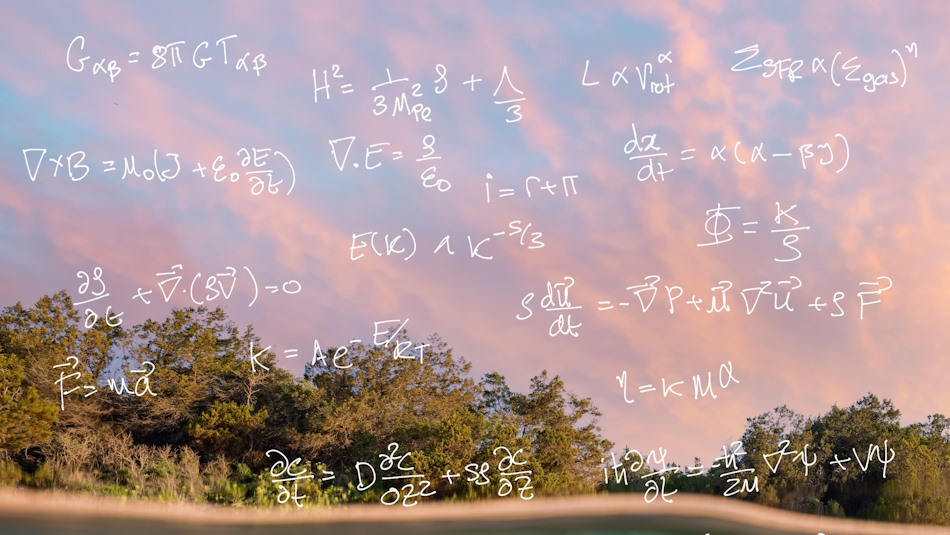
\includegraphics[width=1.0\paperwidth]{background.png}}
    \begin{frame}[plain]
        \begin{mdframed}[tikzsetting={draw=none,fill=white,fill opacity=0.9,
            line width=0pt, align=center},backgroundcolor=none,leftmargin=0,
            rightmargin=0,innertopmargin=4pt]
            {\huge \bfseries \fancyfont Symbolic Regression in the Physical Sciences}\\
            \vspace{2em}

            {\Large \bfseries \color{NavyBlue} \inserttitle}\\
            {\insertauthor}
        \end{mdframed}
    \end{frame}
}

\begin{frame}
    \frametitle{About Me}

    \B{Professor of Data Science and Machine Learning}\\
    University of Applied Sciences Upper Austria\\
    Heuristic and Evolutionary Algorithms Laboratory
    \bigskip

    \B{Research Interests}
    \begin{itemize}
        \item symbolic regression, physical modeling, simulation and optimization
        \item explainability and interpretable machine learning
        \item algorithm design, scalability, energy-efficient AI
        \item chess engine programming
        \item author of the Operon library\\
        \url{https://github.com/heal-research/operon}
    \end{itemize}
\end{frame}

\section{Zobrist Hashing}
\begin{frame}
    \frametitle{Zobrist Hashing}

    \B{Technique used in abstract board games to implement transposition tables.}

    \begin{itemize}
        \item Starts by randomly generating bitstrings for each possible element of a board game\\(i.e. for each combination of a piece and a position)
        \item The Zobrist hash is computed by combining those bitstrings using bitwise XOR
        \item If the bitstrings are long enough, the probability of collisions is negligible
    \end{itemize}
    \bigskip{}

    \B{Bitwise XOR $\to$ incremental hash update}
    \begin{align*}
        a \oplus b &= b \oplus a & & \text{(associativity)}\\
        a \oplus (b \oplus c) &= (a \oplus b) \oplus c & & \text{(commutativity)}\\
        a \oplus b \oplus b &= a & & \text{(involution)}
    \end{align*}
\end{frame}

\begin{frame}
    \frametitle{Zobrist Hashing}

    \AB{Example}

    The word ``cat'' contains three symbols: \A{c}, \A{a}, \A{t}. We associate some random values to each letter:
    \begin{table}
        \centering
        \begin{tblr}{colspec={ll}, stretch=0}
            a & 485\\
            c & 688\\
            t & 118\\
        \end{tblr}
    \end{table}

    \begin{itemize}
        \item $\mathcal{H}(\text{``cat''}) = 688 \oplus 485 \oplus 118 = 803$
        \item hashing lowercase words up to length $m$ from an alphabet of size $n$ will require a $n \times m$ Zobrist table (filled with random values)
        \item \A{for a board game}: $n$ squares $\times$ $m$ piece types \begin{itemize}
            \item Chess: $n=64, m=12$
            \item Go: $n=361, m=2$
            \item \A{Symbolic regression}: (number of symbols) $\times$ (max expression size)
        \end{itemize}
    \end{itemize}
\end{frame}

\begin{frame}
    \frametitle{Zobrist Hashing}

    \begin{columns}[t]
        \column{0.5\textwidth}

        \chessboard[boardfontencoding=LSBC4,setfontcolors,
            setfen={8/8/4kpp1/3p4/p6P/2B4b/6P1/6K1},showmover=true,
            fontsize=12pt,boardfontsize=15]

        \column{0.5\textwidth}

        \begin{table}
            \footnotesize
            \begin{tblr}{colspec={c|ccccc}, column{1}={font=\chessfont\Large}, row{8}={font=\bfseries}, rowsep=1.2pt}
                \whitepawn & 2173 & 1288 & 1235 & 2880 & 3217\\
                \blackpawn & 1074 & 1570 & 3800 & 1538 & 1260\\
                \whiteknight & 3658 & 1022 & 1433 & 1801 & 2504\\
                \blackknight & 4054 & 3302 & 2029 & 1632 & 2549\\
                {\footnotesize $\vdots$} & $\vdots$ & $\vdots$ & $\vdots$ & $\vdots$ & $\vdots$\\
                \whiteking & 1909 & 3847 & 3117 & 2965 & 2533\\
                \blackking & 1270 & 1694 & 1986 & 3800 & 4014\\
                \hline
                & 0 & 1 & 2 & \dots & 63\\
                & $a_1$ & $b_1$ & $c_1$ & \dots & $h_8$\\
            \end{tblr}
        \end{table}
    \end{columns}
    \bigskip

    \[
        \mathcal{H}(\text{position}) = h_{\text{\whiteking}g_1} \oplus h_{\text{\whitepawn}g_2} \oplus h_{\text{\whitebishop}c_3} \oplus h_{\text{\blackbishop}h_3} \oplus h_{\text{\whitepawn}h_4} \oplus h_{\text{\blackpawn}a_4} \oplus h_{\text{\blackpawn}d_5} \oplus h_{\text{\blackking}e_6} \oplus h_{\text{\blackpawn}f_6} \oplus h_{\text{\blackpawn}g_6}
    \]
\end{frame}

\begin{frame}
    \frametitle{Zobrist Hashing}

    \begin{table}
        \centering
        \begin{tblr}{colspec={c|c}, rows={f}}
            \adjustbox{valign=c}{\rotatebox{90}{\hspace{0.7cm}symbol $s \in \mathcal{S}$}} & {Randomly generated\\ hash values $h_{s,i}$}\\
            \hline
            & position $i$\\
        \end{tblr}
    \end{table}

    \[
        \mathcal{H}(\text{state}) = \bigoplus h_{s, i}
    \]

    If the \A{state} of a program$^1$ can be described by a list of symbols and their associated positions, then it can be efficiently maintained using Zobrist hashing.
    \bigskip

    \footnotesize
    $^{1}\text{algorithm, search method, simulation, optimization procedure}$
\end{frame}

\begin{frame}
    \frametitle{Zobrist Hashing}

    \begin{figure}
        \centering
        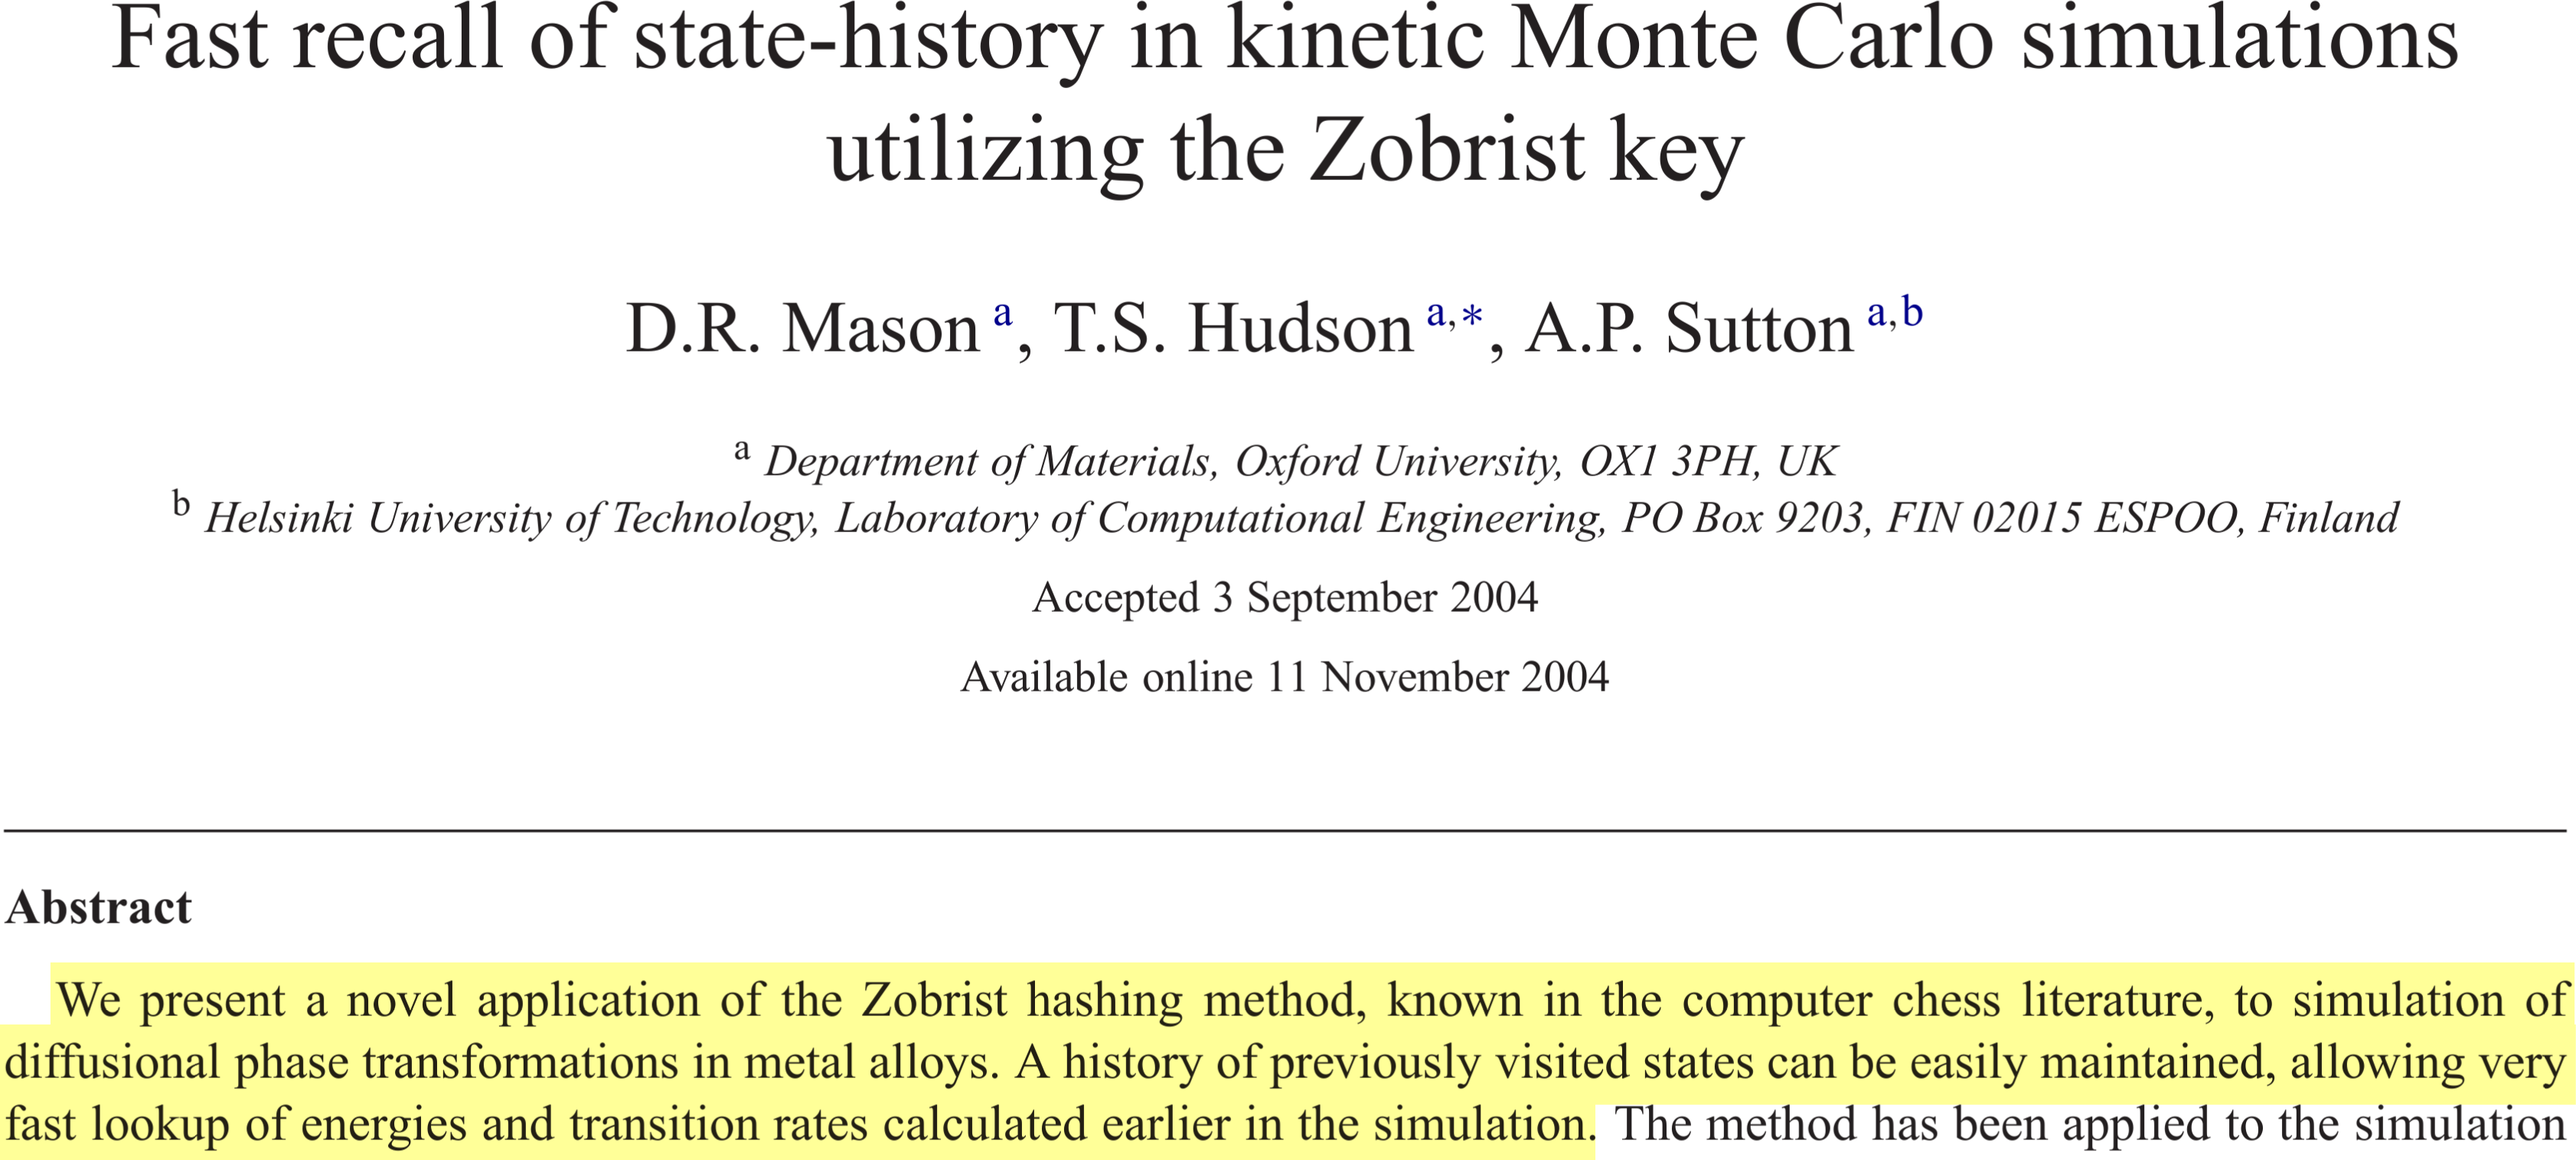
\includegraphics[width=1\textwidth]{./fig/zobrist_monte_carlo.png}
    \end{figure}
\end{frame}


\begin{frame}
    \frametitle{Zobrist Hashing in Symbolic Regression}
    \begin{columns}[t]

    \column{0.5\textwidth}
    Expression tree $T$
    \begin{figure}
        \begin{forest}
            [$^{\color{red} 0}\times$ [$^{\color{red} 1}+$ [$^{\color{red}2}x_1$] [$^{\color{red}3}x_2$]] [$^{\color{red}4}-$ [$^{\color{red}5}x_3$] [$^{\color{red}6}x_4$]]]
        \end{forest}\\
        $f(\mathbf{x}) = (x_1 + x_2) \times (x_3 - x_4)$
    \end{figure}

    Prefix representation:
    \begin{table}
        \begin{tblr}{colspec={ccccccc}, colsep=1.5pt, row{2}={font=\color{red}\scriptsize}, rowsep=0pt}
            $\times$ & $+$ & $x_1$ & $x_2$ & $-$ & $x_3$ & $x_4$\\
            0 & 1 & 2 & 3 & 4 & 5 & 6\\
        \end{tblr}
    \end{table}

    \column{0.5\textwidth}
    Zobrist table:
    \begin{table}
        \footnotesize
        \begin{tblr}{colspec={c|c}, rowsep=1.2pt}
            $+$ & \SetCell[r=9]{c} {Filled with\\ random values}\\
            $-$ & \\
            $\times$ & \\
            $\div$ & \\
            $\vdots$ & \\
            $x_1$ & \\
            $x_2$ & \\
            $x_3$ & \\
            $x_4$ & \\
            $c$   & \\
            \hline
                & position $i = 0,\dots,N$\\
        \end{tblr}
    \end{table}
    \end{columns}

    \centering
    $\mathcal{H}(T) = h_{\times,0} \oplus h_{+, 1} \oplus h_{x_1, 2} \oplus h_{x_2, 3} \oplus h_{-,4} \oplus h_{x_3, 5} \oplus h_{x_4, 6}$
\end{frame}

\begin{frame}
    \frametitle{Zobrist Hashing in Symbolic Regression}

    \begin{figure}
        \centering
        \begin{subfigure}[b]{0.42\textwidth}
            % \caption{Parent $T_1$}
            Parent tree $T_1$\\
            \begin{forest}
                [$^{\color{red} 0}\times$ [$^{\color{red} 1}+$ [$^{\color{red}2}x_1$] [$^{\color{red}3}x_2$]] [$^{\color{red}4}-$, color=Green [$^{\color{red}5}x_3$, color=Green, edge=Green] [$^{\color{red}6}x_4$, color=Green, edge=Green]]]
            \end{forest}\\
            $f_1(\mathbf{x}) = (x_1 + x_2) \times (x_3 - x_4)$
        \end{subfigure}
        \begin{subfigure}[b]{0.29\textwidth}
            Parent tree $T_2$\\
            \begin{forest}
                [$^{\color{red} 0}\div$ [$^{\color{red} 1}\times$ [$^{\color{red}2}x_1$] [$^{\color{red}3}x_2$]] [$^{\color{red}4}\centerdot^2$, color=NavyBlue [$^{\color{red}5}x_3$, color=NavyBlue, edge=NavyBlue]]]
            \end{forest}\\
            $f_2(\mathbf{x}) = {x_1 x_2}/{x_3^2}$
        \end{subfigure}
        \begin{subfigure}[b]{0.25\textwidth}
            Child tree $C_1$\\
            \begin{forest}
                [$^{\color{red} 0}\times$ [$^{\color{red} 1}+$ [$^{\color{red}2}x_1$] [$^{\color{red}3}x_2$]] [$^{\color{red}4}\centerdot^2$, color=NavyBlue [$^{\color{red}5}x_3$, color=NavyBlue, edge=NavyBlue]]]
            \end{forest}\\
            $f_3(\mathbf{x}) = (x_1 + x_2){x_3^2}$
        \end{subfigure}
    \end{figure}
    \bigskip

    \A{Incremental hash update after crossover}
    \[
        \mathcal{H}(C_1) = \mathcal{H}(T_1) \oplus {\color{Green}\underbrace{h_{-,4} \oplus h_{x_3,5} \oplus h_{x_4, 6}}_{\text{XOR ``out'' $(x_3 - x_4)$}}} \oplus {\color{NavyBlue} \underbrace{h_{\centerdot^2,4} \oplus  h_{x_3, 5}}_{\text{XOR ``in'' $x_3^2$}}}
    \]
\end{frame}

\begin{frame}
    \frametitle{Zobrist Hashing in Symbolic Regression}

    \B{The Zobrist hash provides a means to cache duplicate structures that may occur}
    \begin{itemize}
        \item We could cache solution candidates and their fitness
        \item We could use this information to guide the search
    \end{itemize}
    \bigskip

    \BB{Why do duplicates occur in the first place?}
    \begin{itemize}
        \item The search process is driven by ``natural selection''
        \item Selection probability proportional with fitness (i.e., training error)
        \item Fit solution candidates will propagate (``survival of the fittest'')
    \end{itemize}
\end{frame}


\begin{frame}
    \frametitle{Zobrist Hashing in Symbolic Regression}

    \begin{figure}
        \tcbset{enhanced, width=0.9\textwidth, nobeforeafter, rounded corners, arc=1mm, colbacktitle=NavyBlue, coltitle=white, fonttitle=\bfseries, colback=gray!10!white}

        \begin{tcolorbox}[title=Initialization, remember as=N1]
            \begin{enumerate}
                \item Generate $N$ random trees
                \item Evaluate their fitness on the training data
            \end{enumerate}
        \end{tcolorbox}
        \vspace{2em}

        \begin{tcolorbox}[title=Main loop, remember as=N2]
            \begin{enumerate}
                \item \textbf{Selection}: choose $N$ parent pairs for recombination
                \item \textbf{Recombination}: produce $N$ children via crossover/mutation
                \item \textbf{Fitness evaluation}: compute fitness for child individuals
                \item \textbf{Replacement}: child individuals replace parents
                \item \textbf{Check stop}: if not converged, go to step 1, otherwise stop.
            \end{enumerate}
        \end{tcolorbox}
        \tikz[overlay, remember picture] \draw[-stealth, line width=3pt, color=gray] (N1)--(N2);
    \end{figure}
\end{frame}

\begin{frame}
    \frametitle{Zobrist Hashing in Symbolic Regression}

    \begin{figure}
        \tcbset{enhanced, width=0.9\textwidth, nobeforeafter, rounded corners, arc=1mm, colbacktitle=NavyBlue, coltitle=white, fonttitle=\bfseries, colback=gray!10!white}

        \begin{tcolorbox}[title=Initialization, remember as=N1]
            \begin{enumerate}
                \item Generate $N$ random trees
                \item Evaluate their fitness on the training data
            \end{enumerate}
        \end{tcolorbox}
        \vspace{2em}

        \begin{tcolorbox}[title=Main loop, remember as=N2]
            \begin{enumerate}
                \item \textbf{Selection}: choose $N$ parent pairs for recombination
                \item \textbf{Recombination}: produce $N$ children via crossover/mutation $\implies$ \hlcyan{promote novelty}
                \item \textbf{Fitness evaluation}: compute fitness for child individuals $\implies$\hlcyan{cache fitness}
                \item \textbf{Replacement}: child individuals replace parents
                \item \textbf{Check stop}: if not converged, go to step 1, otherwise stop.
            \end{enumerate}
        \end{tcolorbox}
        \tikz[overlay, remember picture] \draw[-stealth, line width=3pt, color=gray] (N1)--(N2);
    \end{figure}
\end{frame}

\begin{frame}
    \frametitle{Zobrist Hashing in Symbolic Regression}

    \BB{Novelty promotion}

    If a child individual's Zobrist signature is already in the cache, discard it and produce a new one
    \A{Crossover}: \begin{itemize}
        \item check all possible subtree exchanges between two parent trees $T_1$ and $T_2$
        \item discard exchanges which would lead to an already-seen hash
    \end{itemize}
    \smallskip

    \A{Mutation}:
    \begin{itemize}
        \item for a parent tree $T_1$, perform a random change and update hash, discard already-seen hashes
    \end{itemize}
    \bigskip

    \BB{Fitness cache}

    If child Zobrist hash already in the cache, return stored fitness (do not re-evaluate)
\end{frame}

\begin{frame}
    \frametitle{Zobrist Hashing in Symbolic Regression}

    \BB{Implementation (Operon C++)}
    \begin{itemize}
        \item Global Zobrist table (singleton class) initialized at program start
        \item Parallel hash table mapping Zobrist signature to fitness values
    \end{itemize}
    \bigskip

    \begin{table}
        \footnotesize
        \begin{tblr}{colspec={c|c}, rowsep=1.2pt}
            $+$ & \SetCell[r=9]{c} {Filled with\\ random values}\\
            $-$ & \\
            $\times$ & \\
            $\div$ & \\
            $\vdots$ & \\
            $x_1$ & \\
            $x_2$ & \\
            $x_3$ & \\
            $x_4$ & \\
            $c$   & \\
            \hline
                & position $i = 0,\dots,N$\\
        \end{tblr}
    \end{table}
\end{frame}

\begin{frame}
    \frametitle{Zobrist Hashing in Symbolic Regression}

    \BB{Implementation (Operon C++)}
    \begin{itemize}
        \item Global Zobrist table (singleton class) initialized at program start
        \item Parallel hash table mapping Zobrist signature to fitness values
    \end{itemize}
    \bigskip

    \A{Model coefficients not included in hash signature $\to$ must be optimized beforehand}

    \begin{forest}
        [$+$ [${\color{NavyBlue} \theta_1} x_1$] [${\color{NavyBlue} \theta_2}$]]
    \end{forest}
    \bigskip

    \A{Coefficient optimization}:
    \begin{itemize}
        \item Nonlinear least squares (Levenberg-Marquardt)
        \item Configurable number of gradient descent iterations
    \end{itemize}
\end{frame}

\begin{frame}
    \frametitle{Test problems}

    \begin{table}
        \begin{tblr}{colspec={lrrrr}}
            \AB{Problem} & \AB{Points} & \AB{Features} & \AB{Train} & \AB{Test}\\
            Chemical-I & 4999 & 25 & 3136 & 1863\\
            Chemical-II & 1066 & 57 & 711 & 355\\
            FrictionDyn-OneHot & 2016 & 17 & 1010 & 1016\\
            FrictionStat-OneHot & 2016 & 16 & 1010 & 1016\\
            Flow Stress & 7800 & 2 & 4200 & 3600\\
            Nasa Battery 1\_10 & 636 & 6 & 504 & 132\\
            Nasa Battery 2\_10 & 1638 & 5 & 1101 & 537\\
            Nikuradse 1 & 362 & 2 & 230 & 132\\
            Nikuradse 2 & 362 & 1 & 230 & 132\\
        \end{tblr}
    \end{table}
\end{frame}

\begin{frame}
    \frametitle{Experimental Setup}

    \AB{NSGA-II Algorithm}
    \begin{itemize}
        \item 50 independent runs for each problem
        \item 1000 individuals, 300 generations
        \item varying number of LM-iterations (1, 10, 50, 100)
        \item transposition cache=on/off, transposition-operators=on/off
        \item executed on 16 threads (Ryzen 5950X)
    \end{itemize}
\end{frame}

\begin{frame}
    \frametitle{Preliminary Results -- Runtime}

    \begin{figure}
        \centering
        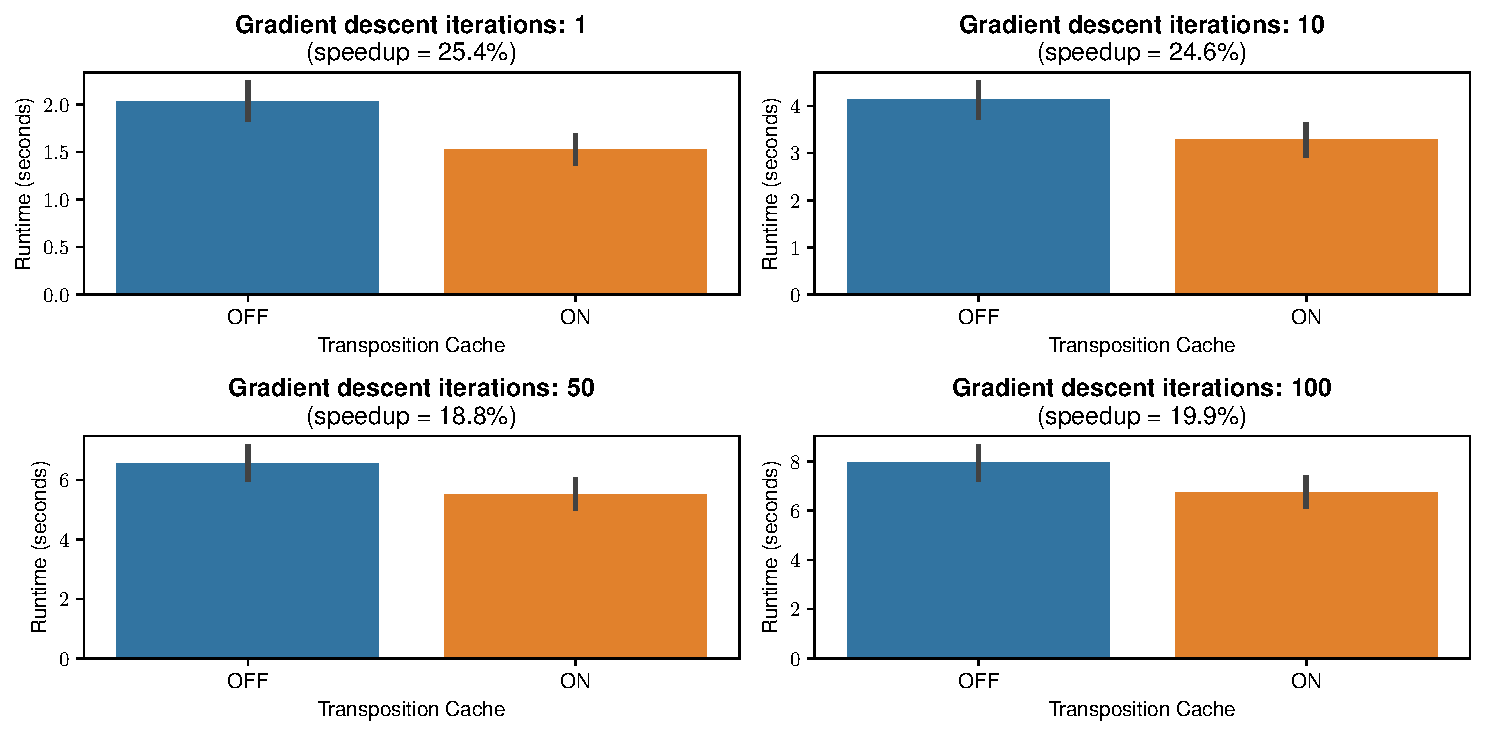
\includegraphics[width=1.0\textwidth]{./fig/runtime.pdf}
    \end{figure}
\end{frame}

\begin{frame}
    \frametitle{Preliminary Results -- Energy Cost}

    \begin{figure}
        \centering
        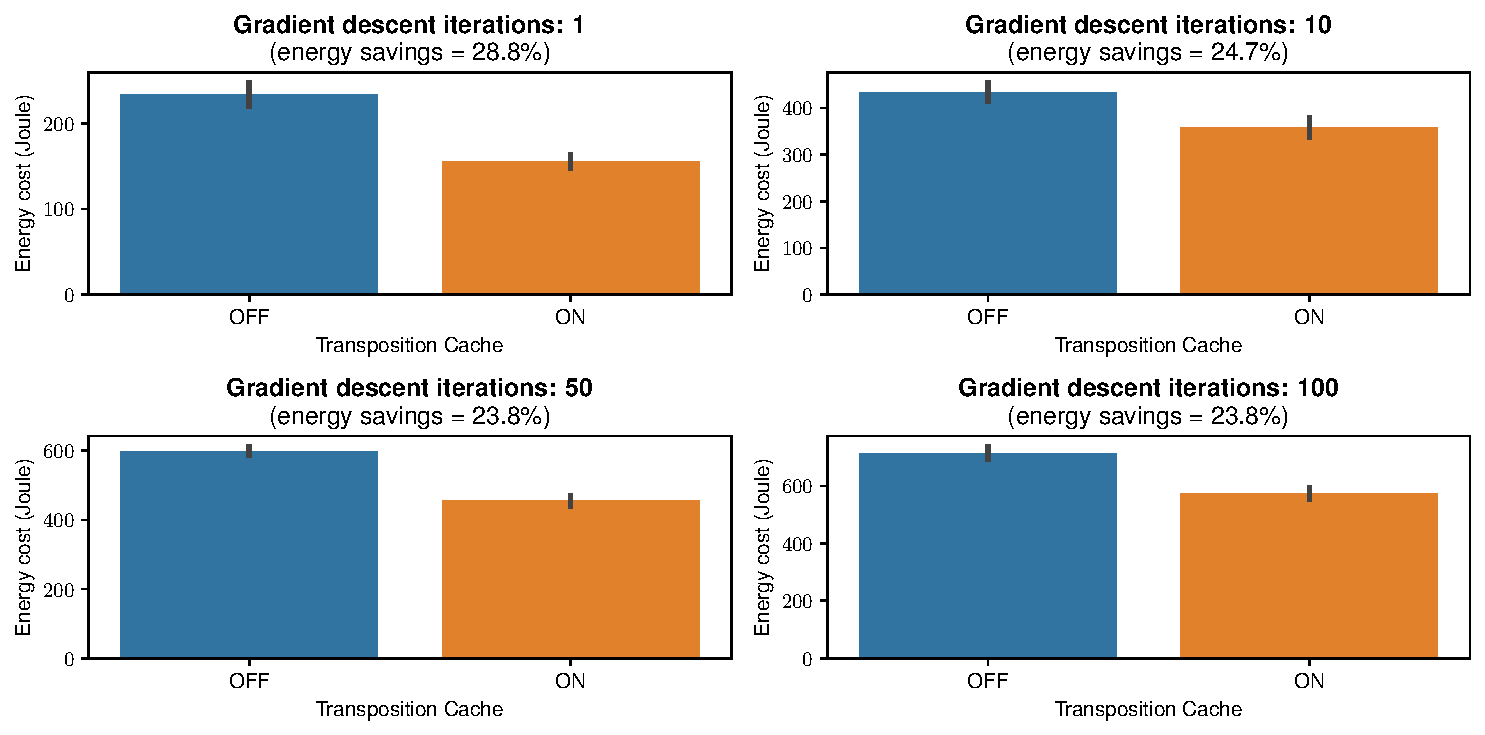
\includegraphics[width=1.0\textwidth]{./fig/energy.pdf}
    \end{figure}
\end{frame}

\begin{frame}
    \frametitle{Preliminary Results}

    \begin{figure}
        \centering
        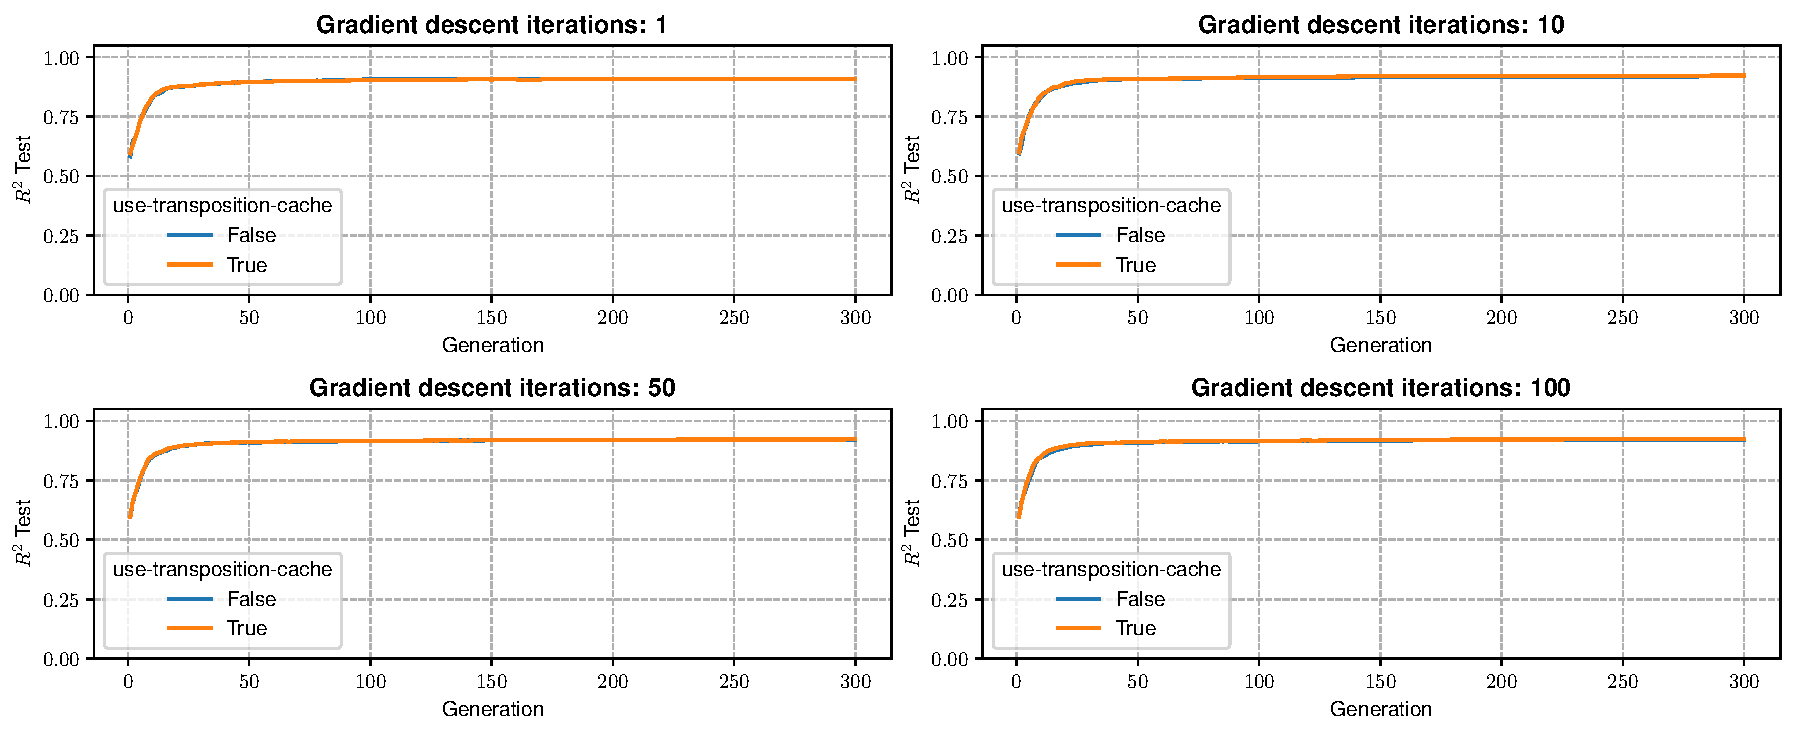
\includegraphics[width=\textwidth]{./fig/Chemical-I_test_performance.pdf}
        \caption{Chemical-I Test Performance}
    \end{figure}
\end{frame}

\begin{frame}
    \frametitle{Preliminary Results}

    \begin{figure}
        \centering
        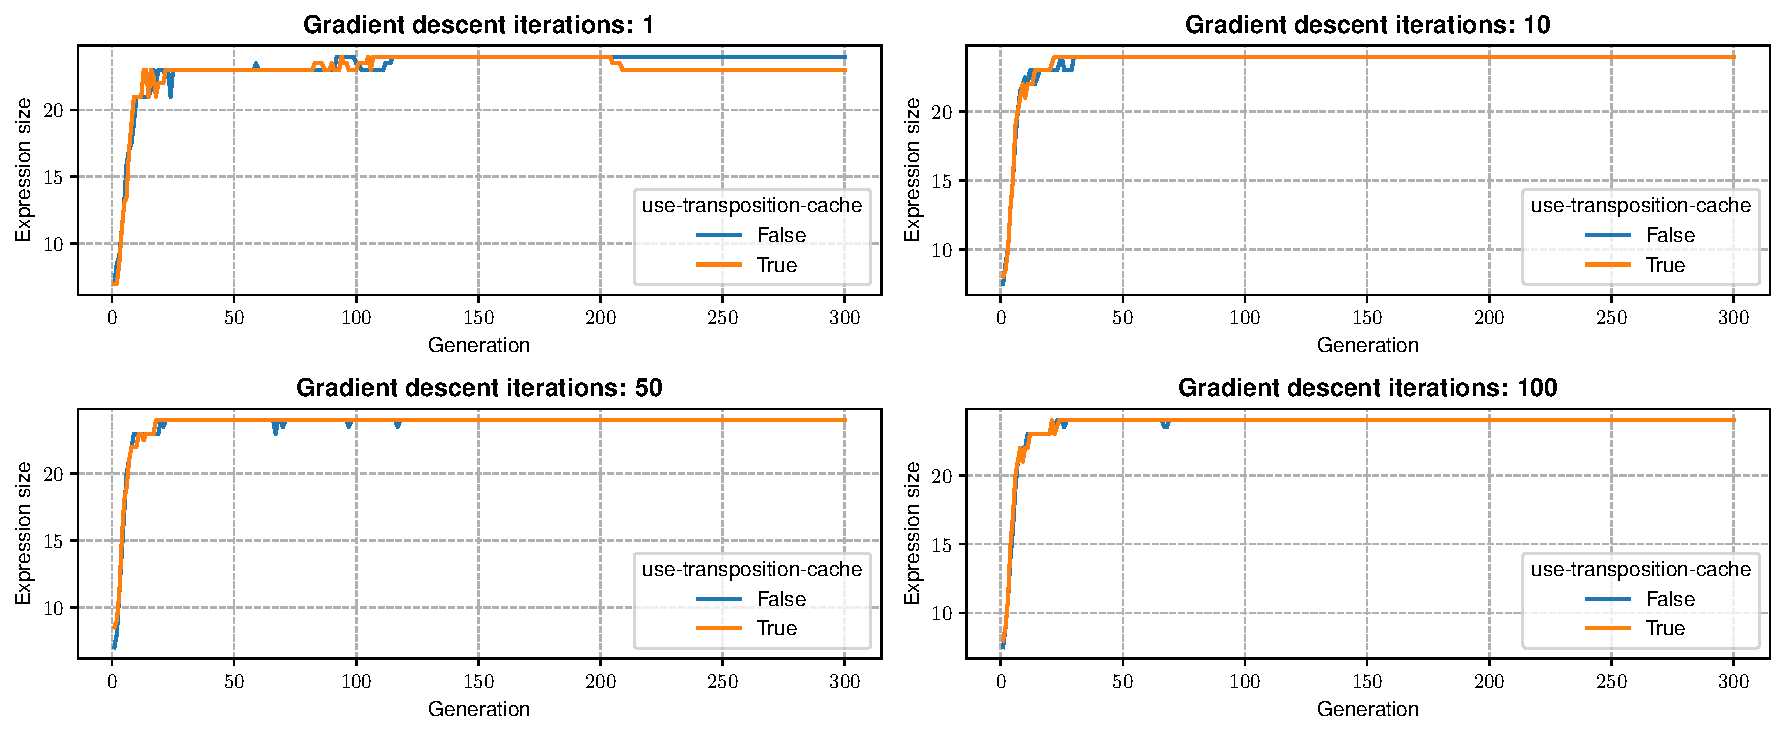
\includegraphics[width=\textwidth]{./fig/Chemical-I_expression_size.pdf}
        \caption{Chemical-I Expression Size}
    \end{figure}
\end{frame}

\begin{frame}
    \frametitle{Preliminary Results}

    \begin{figure}
        \centering
        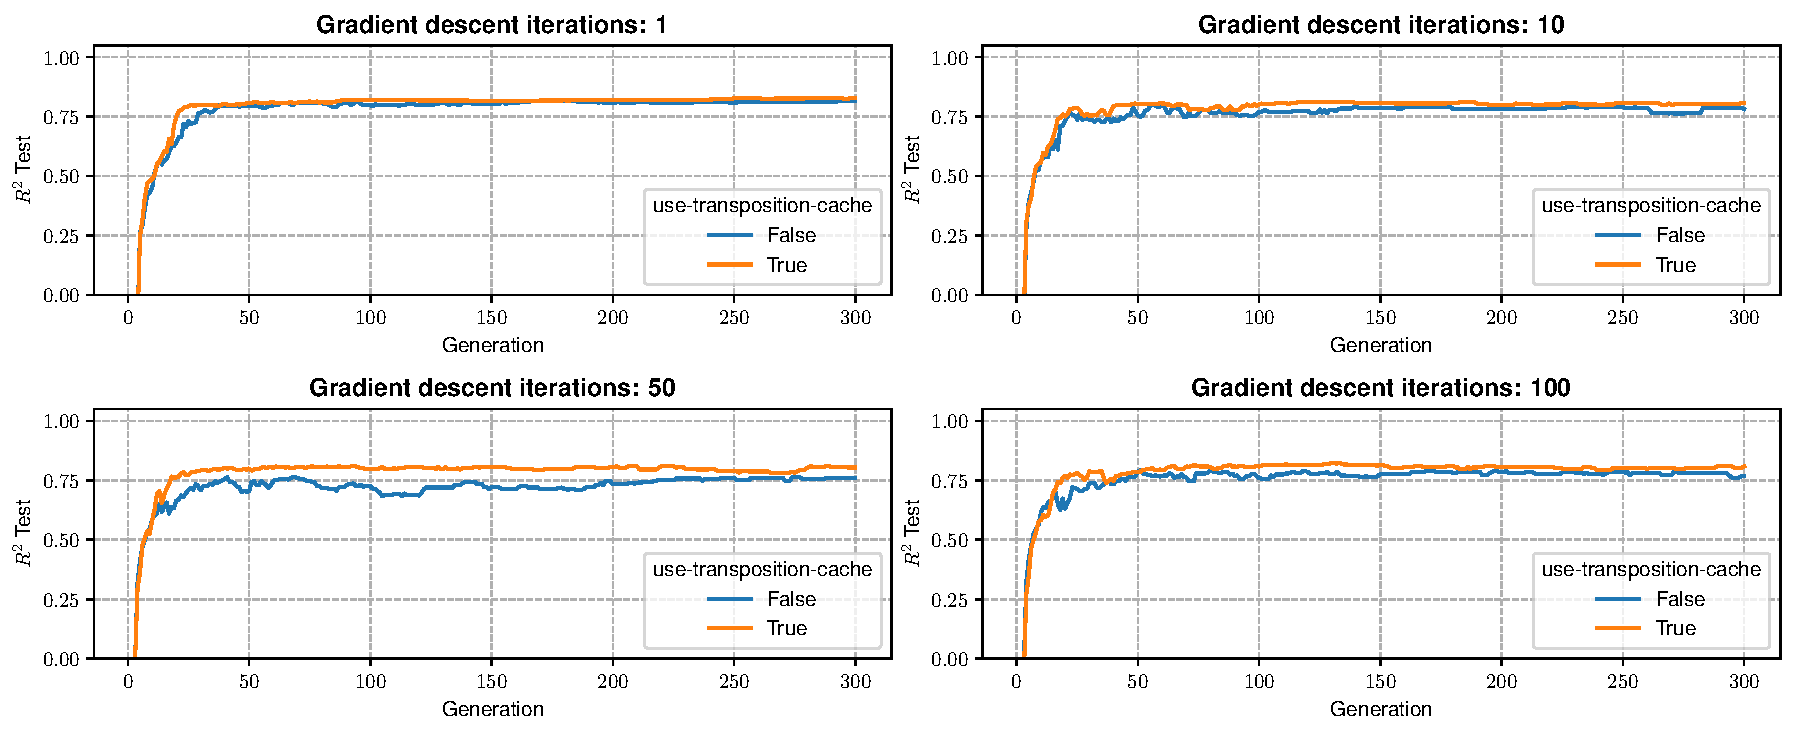
\includegraphics[width=\textwidth]{./fig/Chemical-II_test_performance.pdf}
        \caption{Chemical-II Test Performance}
    \end{figure}
\end{frame}

\begin{frame}
    \frametitle{Preliminary Results}

    \begin{figure}
        \centering
        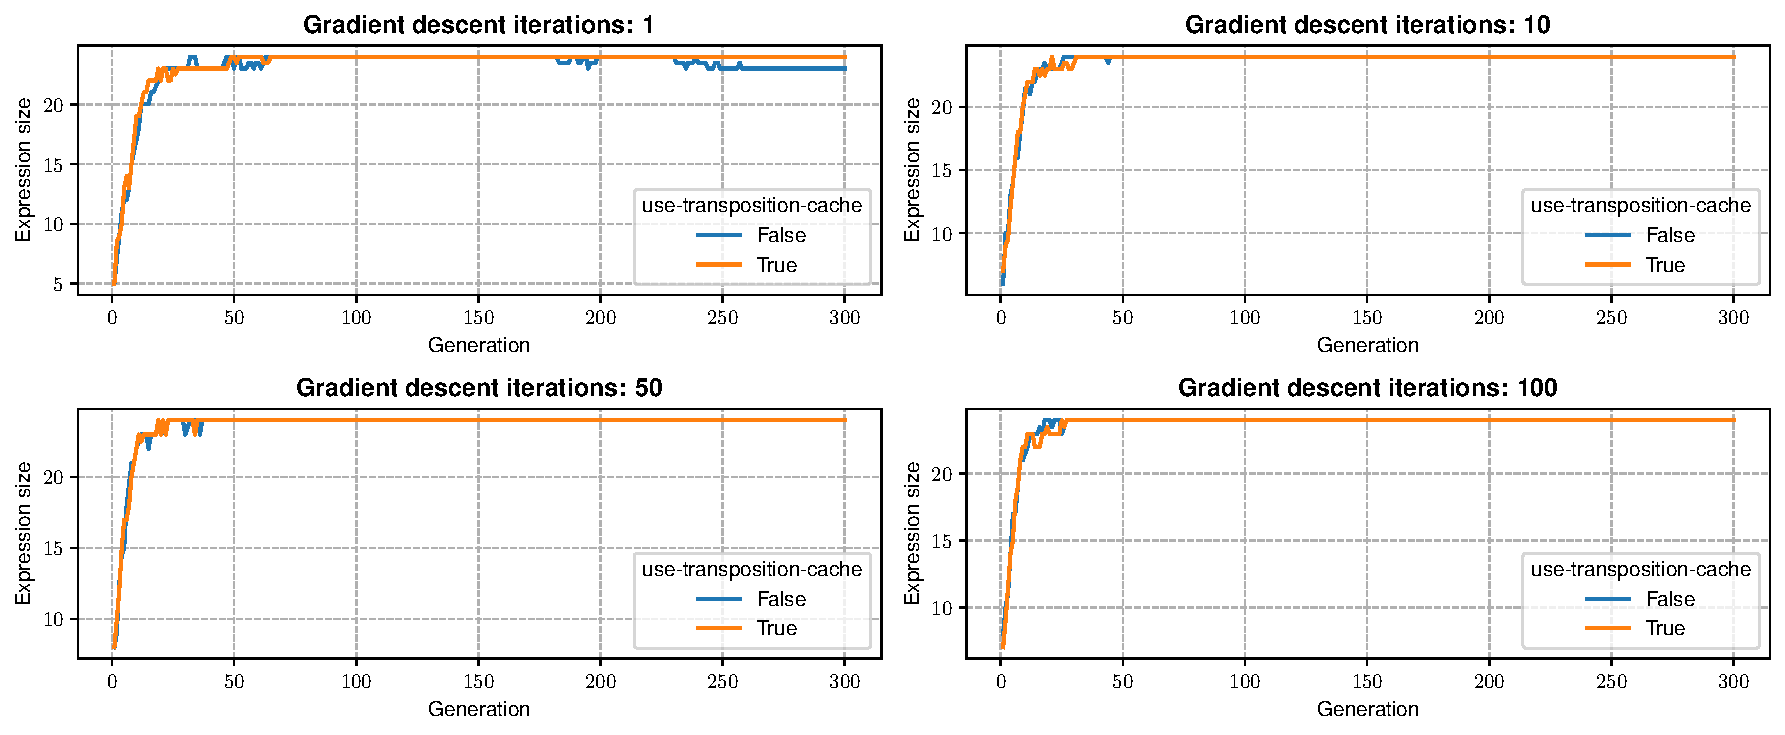
\includegraphics[width=\textwidth]{./fig/Chemical-II_expression_size.pdf}
        \caption{Chemical-II Expression Size}
    \end{figure}
\end{frame}

\begin{frame}
    \frametitle{Preliminary Results}

    \begin{figure}
        \centering
        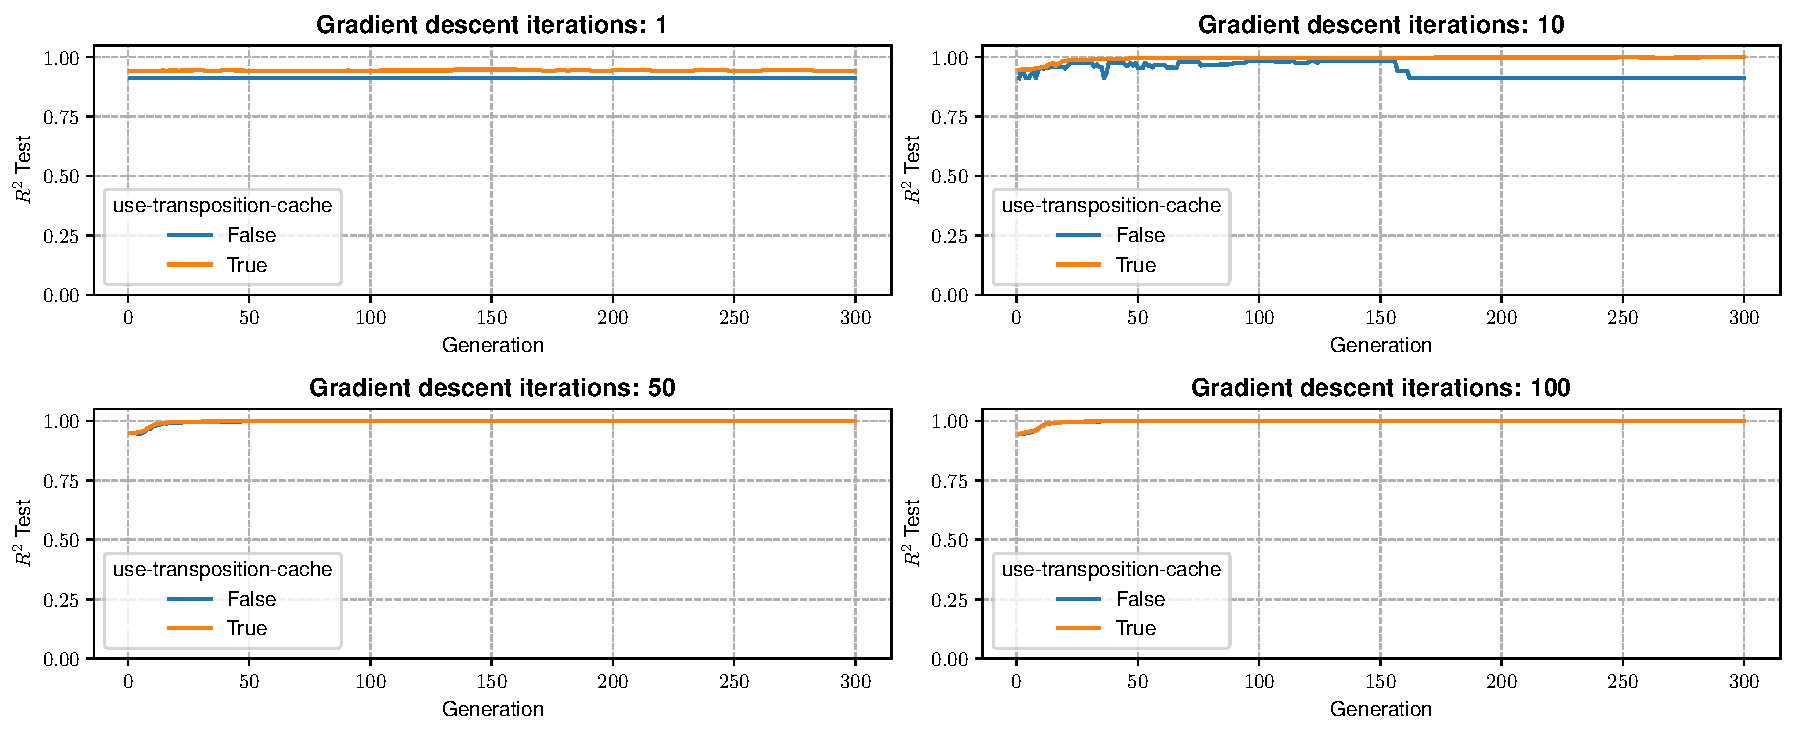
\includegraphics[width=\textwidth]{./fig/Flow-stress_test_performance.pdf}
        \caption{Flow Stress Test Performance}
    \end{figure}
\end{frame}

\begin{frame}
    \frametitle{Preliminary Results}

    \begin{figure}
        \centering
        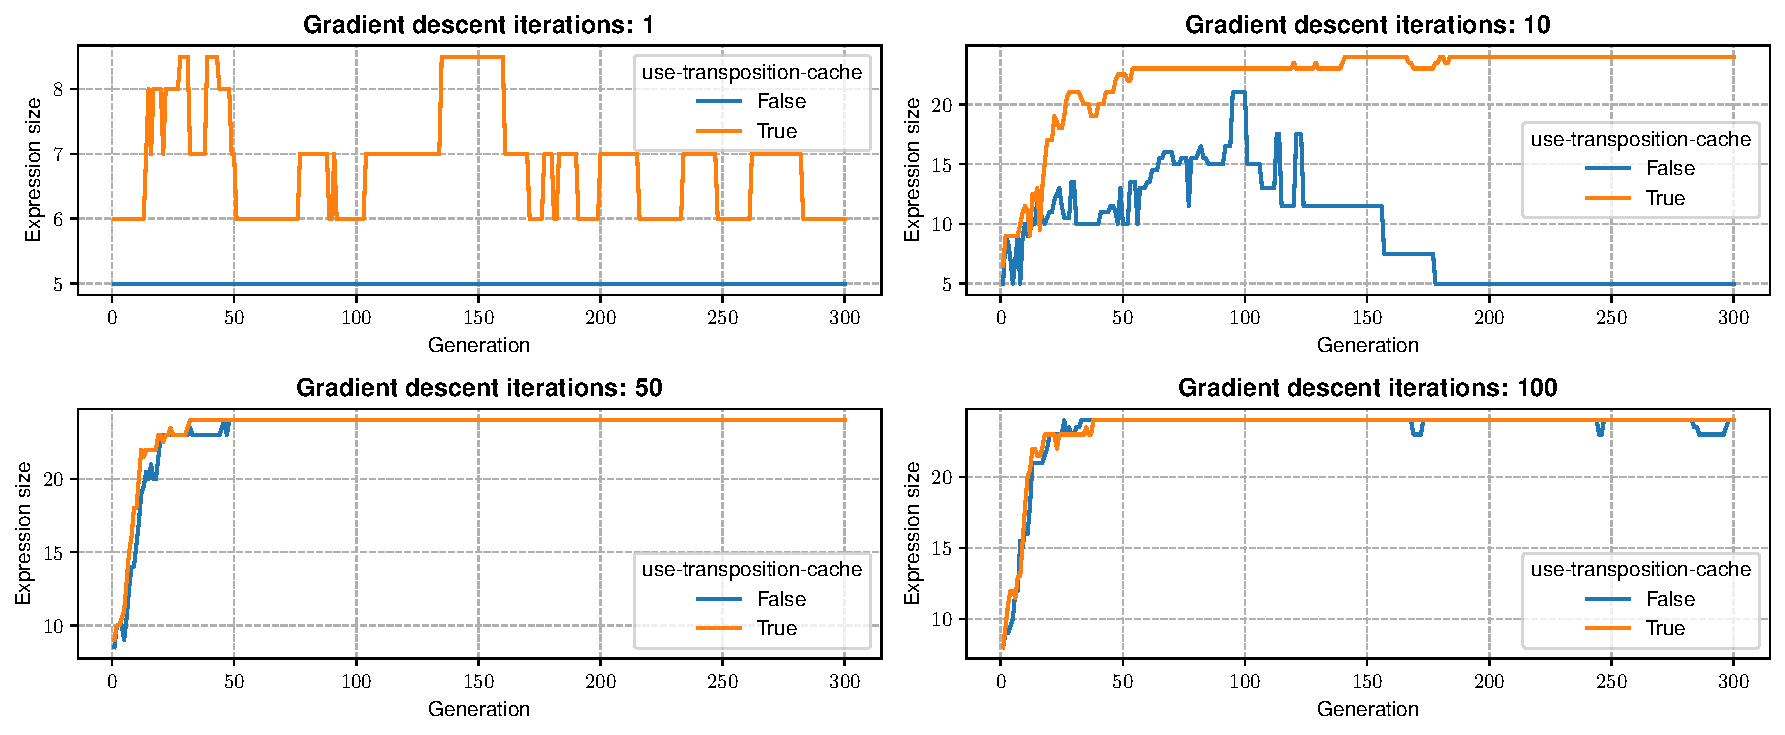
\includegraphics[width=\textwidth]{./fig/Flow-stress_expression_size.pdf}
        \caption{Flow Stress Expression Size}
    \end{figure}
\end{frame}

\begin{frame}
    \frametitle{Preliminary Results}

    \begin{figure}
        \centering
        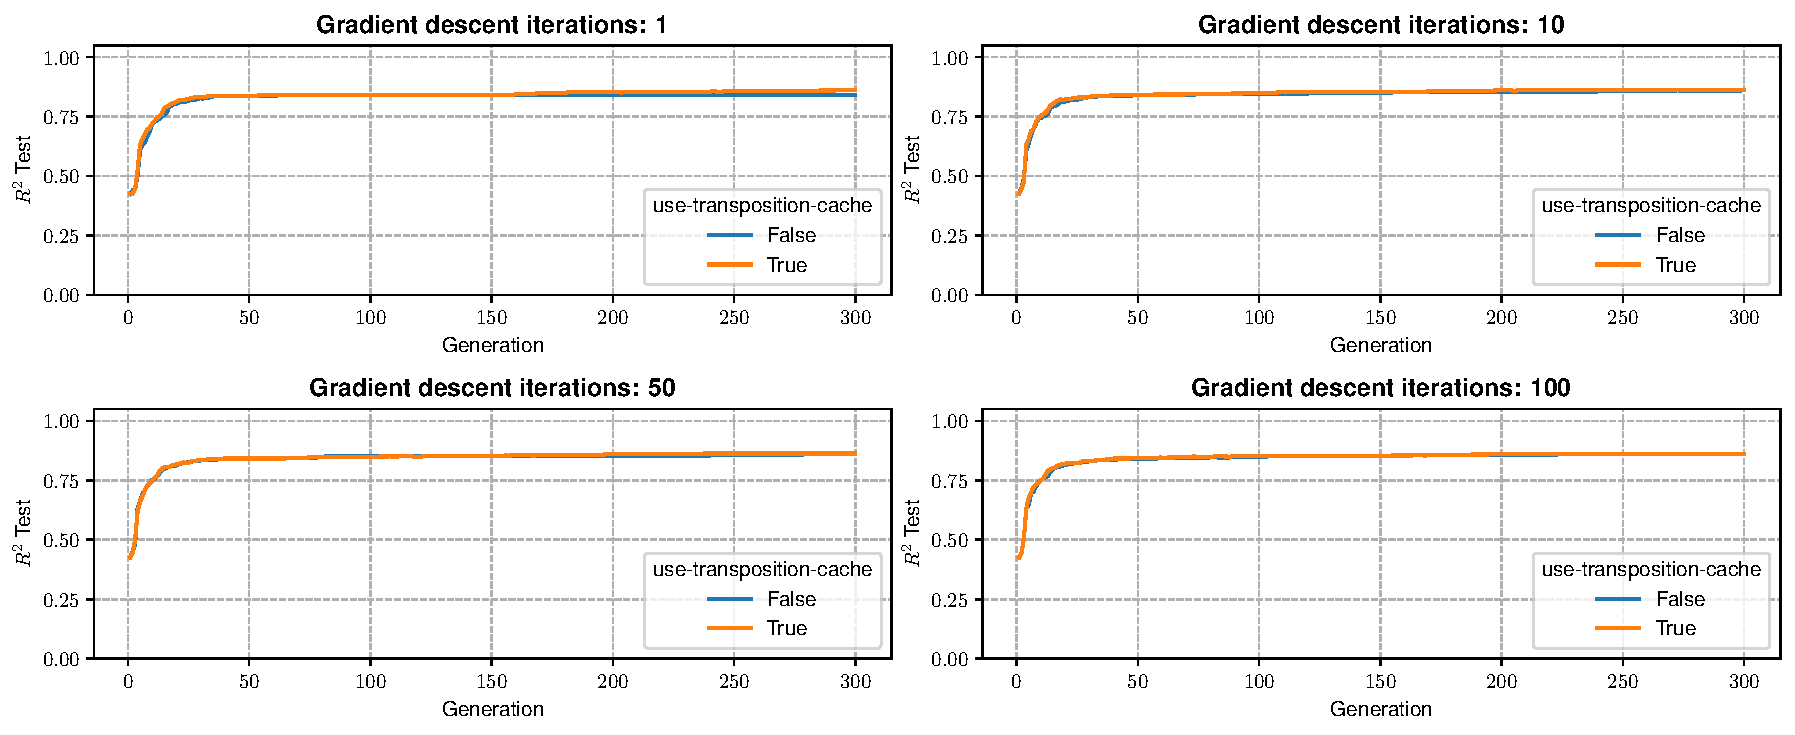
\includegraphics[width=\textwidth]{./fig/FrictionDyn-OneHot_test_performance.pdf}
        \caption{FrictionDyn-OneHot Test Performance}
    \end{figure}
\end{frame}

\begin{frame}
    \frametitle{Preliminary Results}

    \begin{figure}
        \centering
        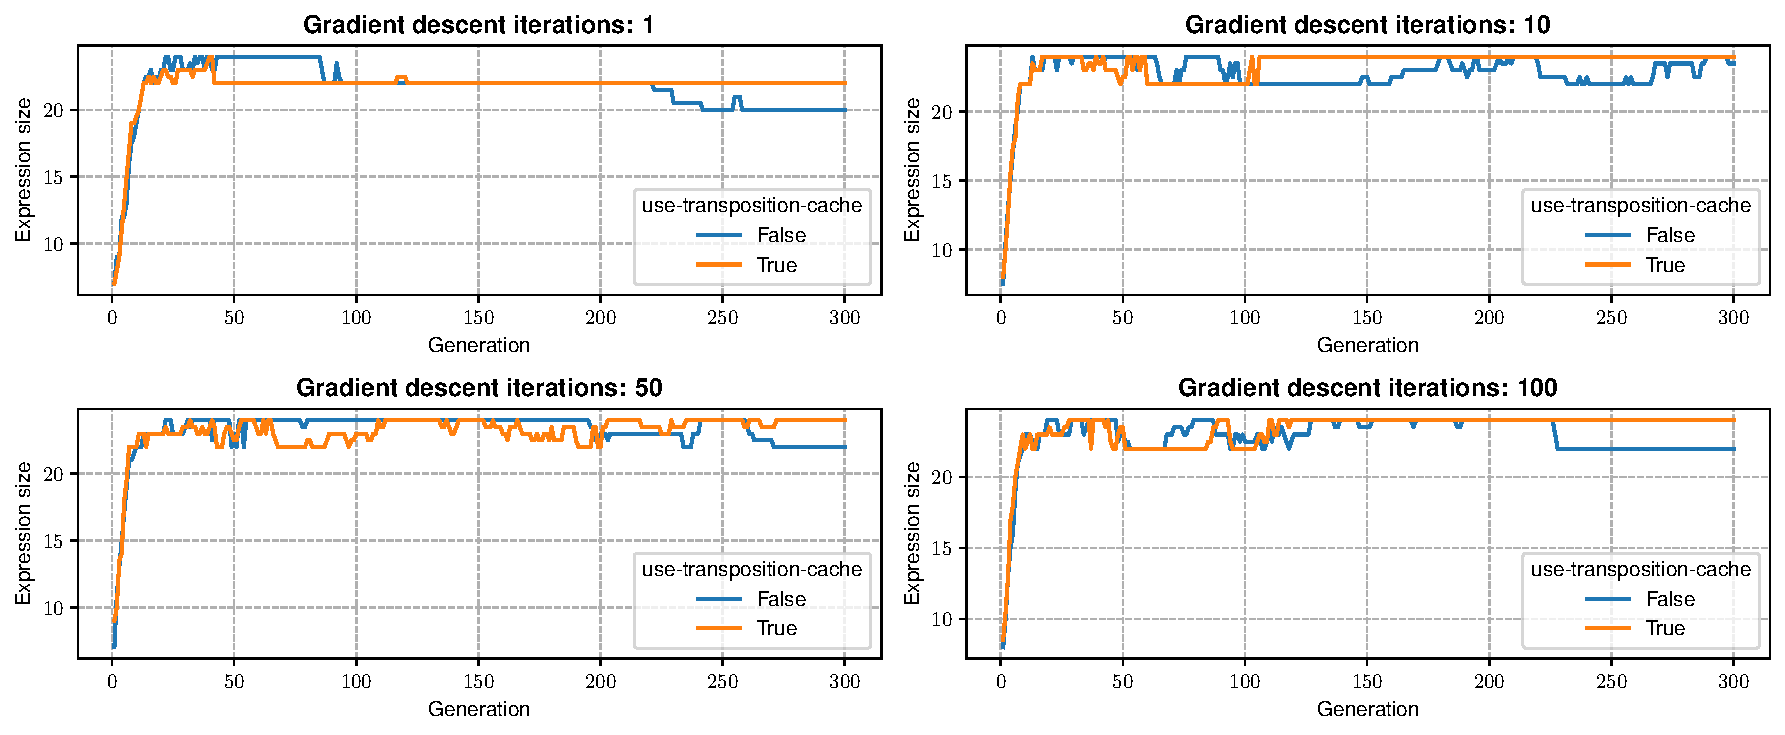
\includegraphics[width=\textwidth]{./fig/FrictionDyn-OneHot_expression_size.pdf}
        \caption{FrictionDyn-OneHot Expression Size}
    \end{figure}
\end{frame}

\begin{frame}
    \frametitle{Preliminary Results}

    \begin{figure}
        \centering
        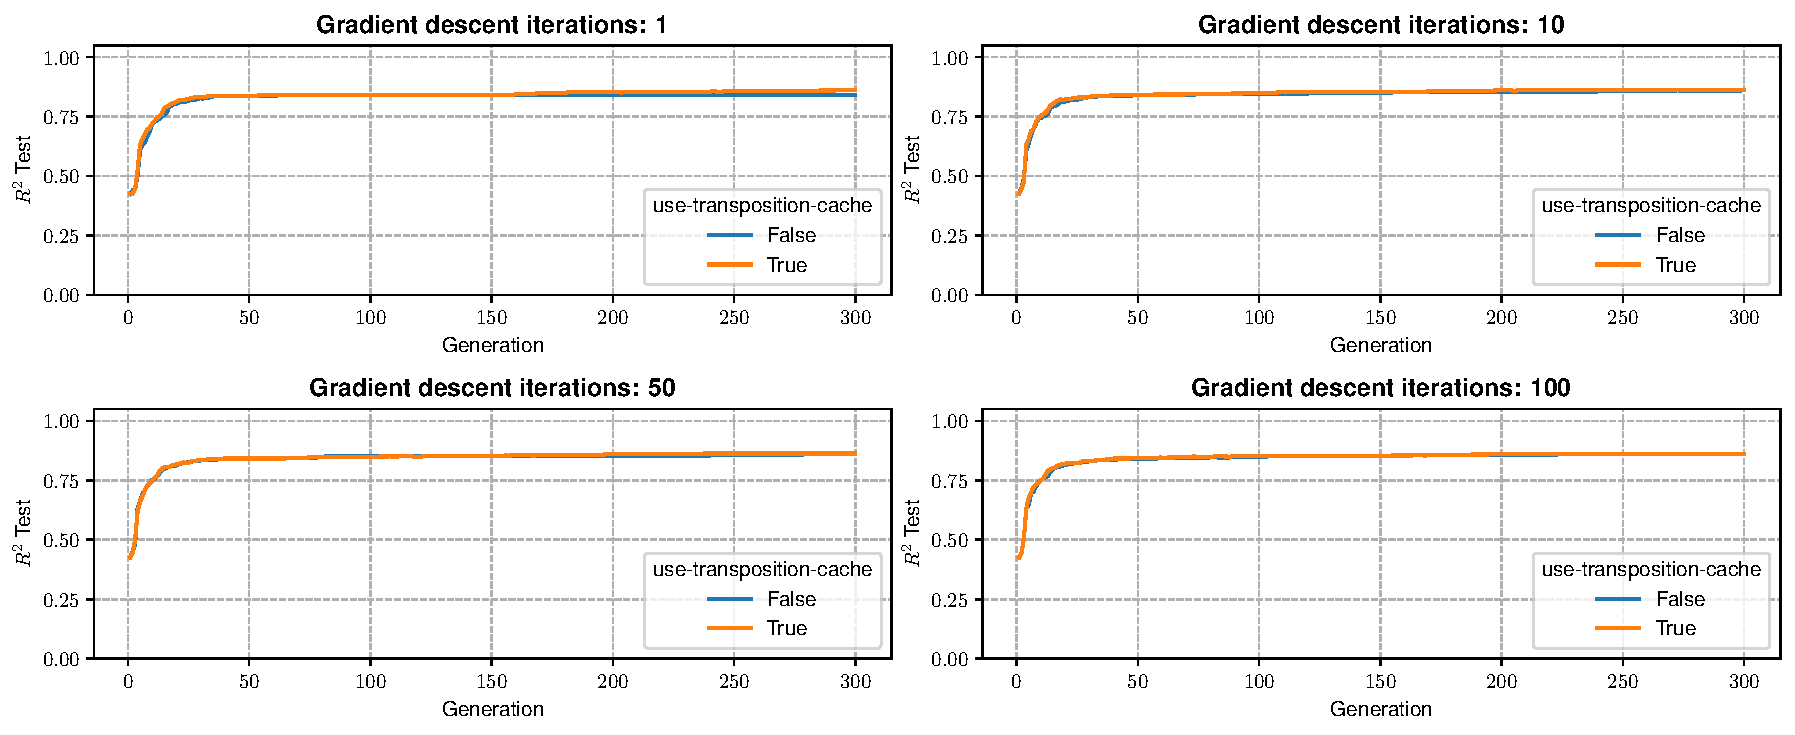
\includegraphics[width=\textwidth]{./fig/FrictionDyn-OneHot_test_performance.pdf}
        \caption{FrictionStat-OneHot Test Performance}
    \end{figure}
\end{frame}

\begin{frame}
    \frametitle{Preliminary Results}

    \begin{figure}
        \centering
        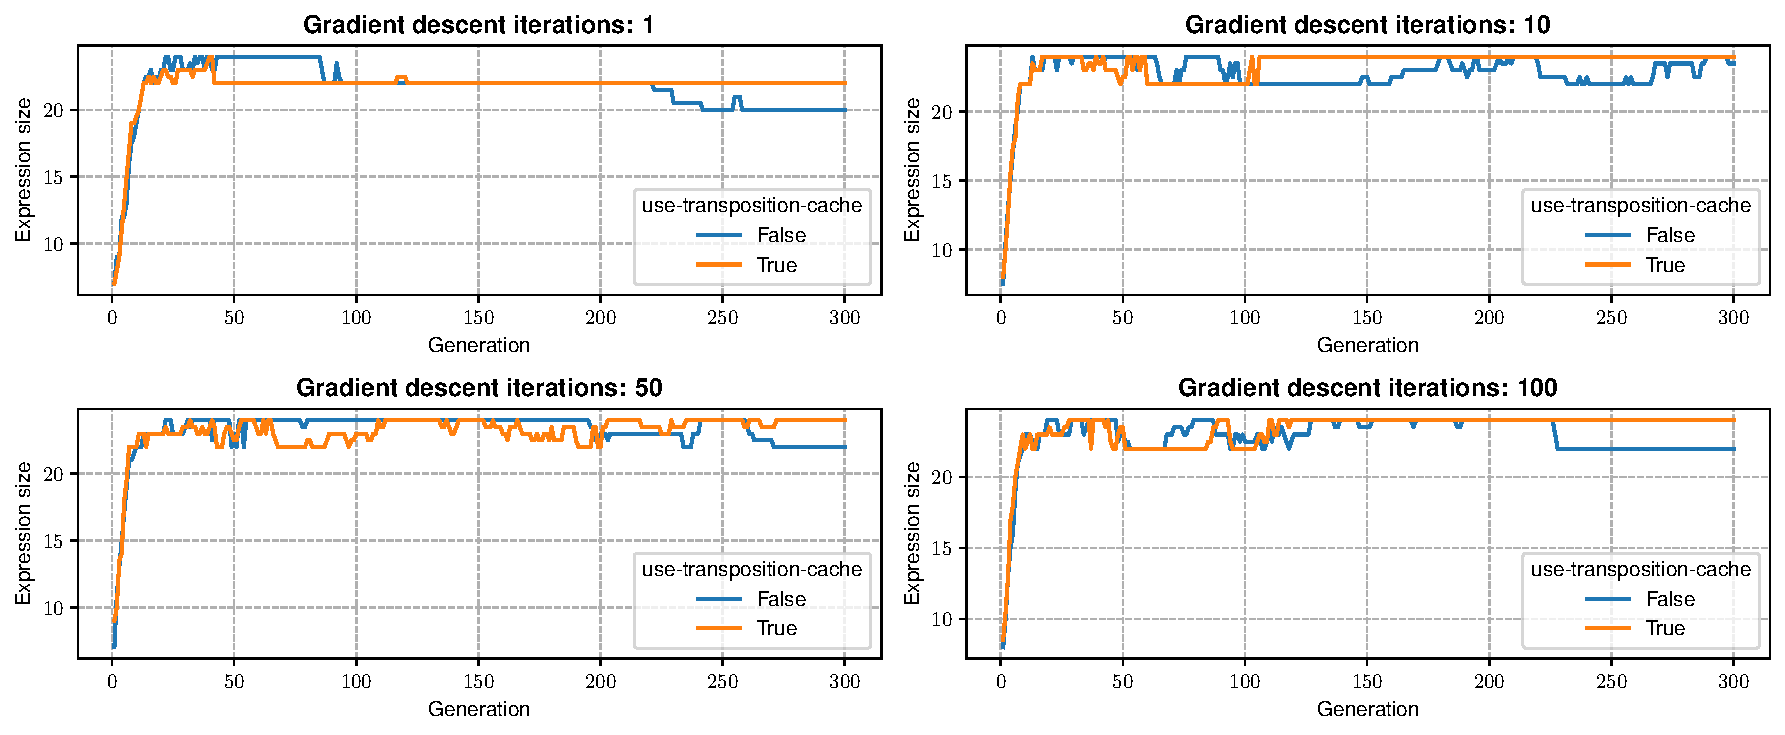
\includegraphics[width=\textwidth]{./fig/FrictionDyn-OneHot_expression_size.pdf}
        \caption{FrictionStat-OneHot Expression Size}
    \end{figure}
\end{frame}

\begin{frame}
    \frametitle{Preliminary Results}

    \begin{figure}
        \centering
        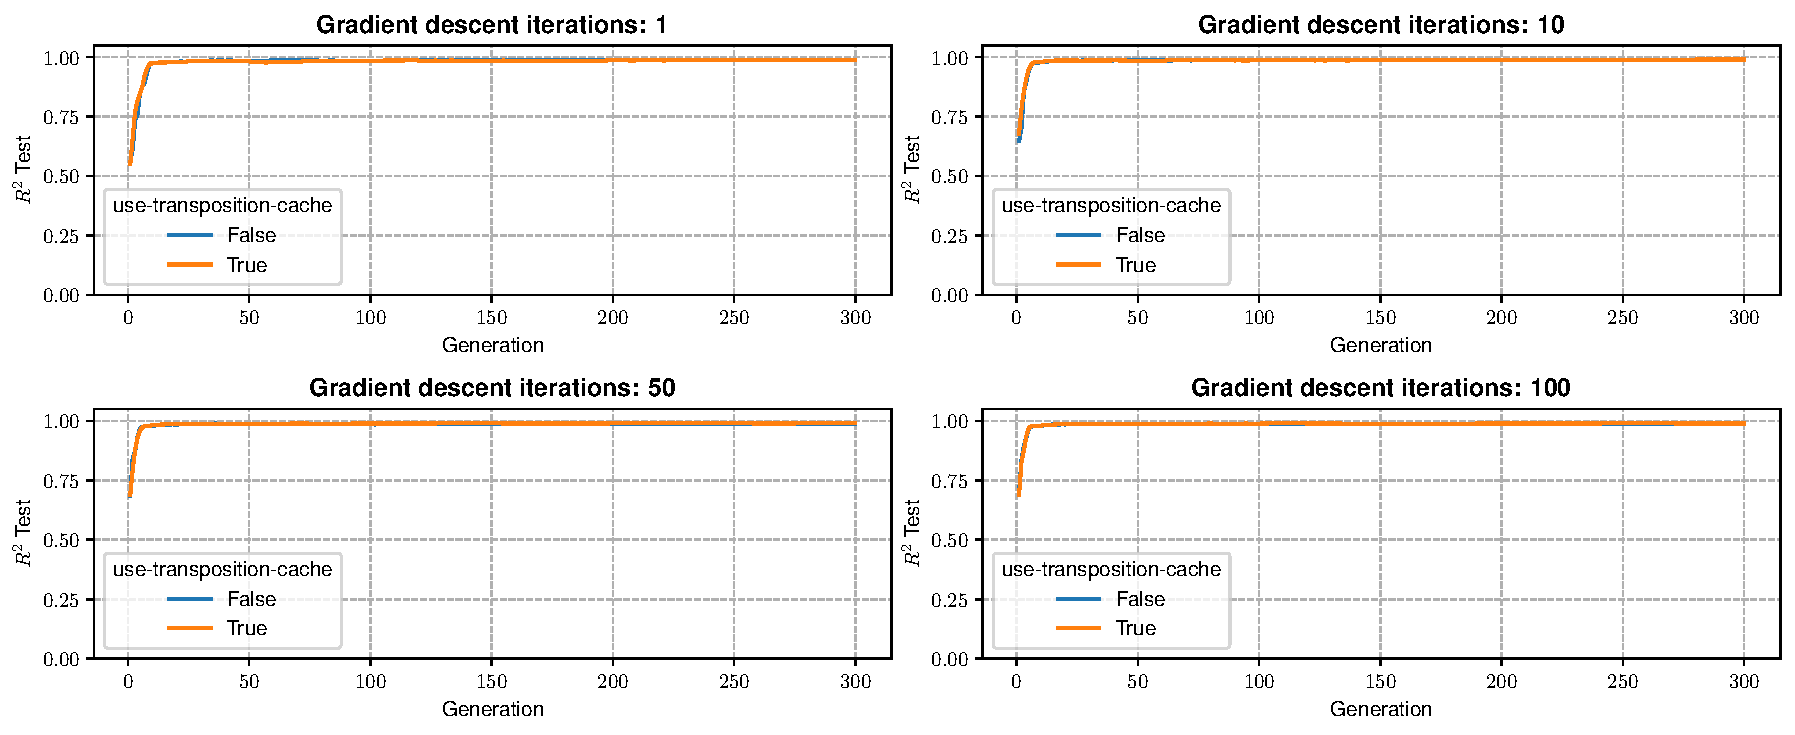
\includegraphics[width=\textwidth]{./fig/Nasa Battery 1_10_test_performance.pdf}
        \caption{Nasa Battery 1\_10 Test Performance}
    \end{figure}
\end{frame}

\begin{frame}
    \frametitle{Preliminary Results}

    \begin{figure}
        \centering
        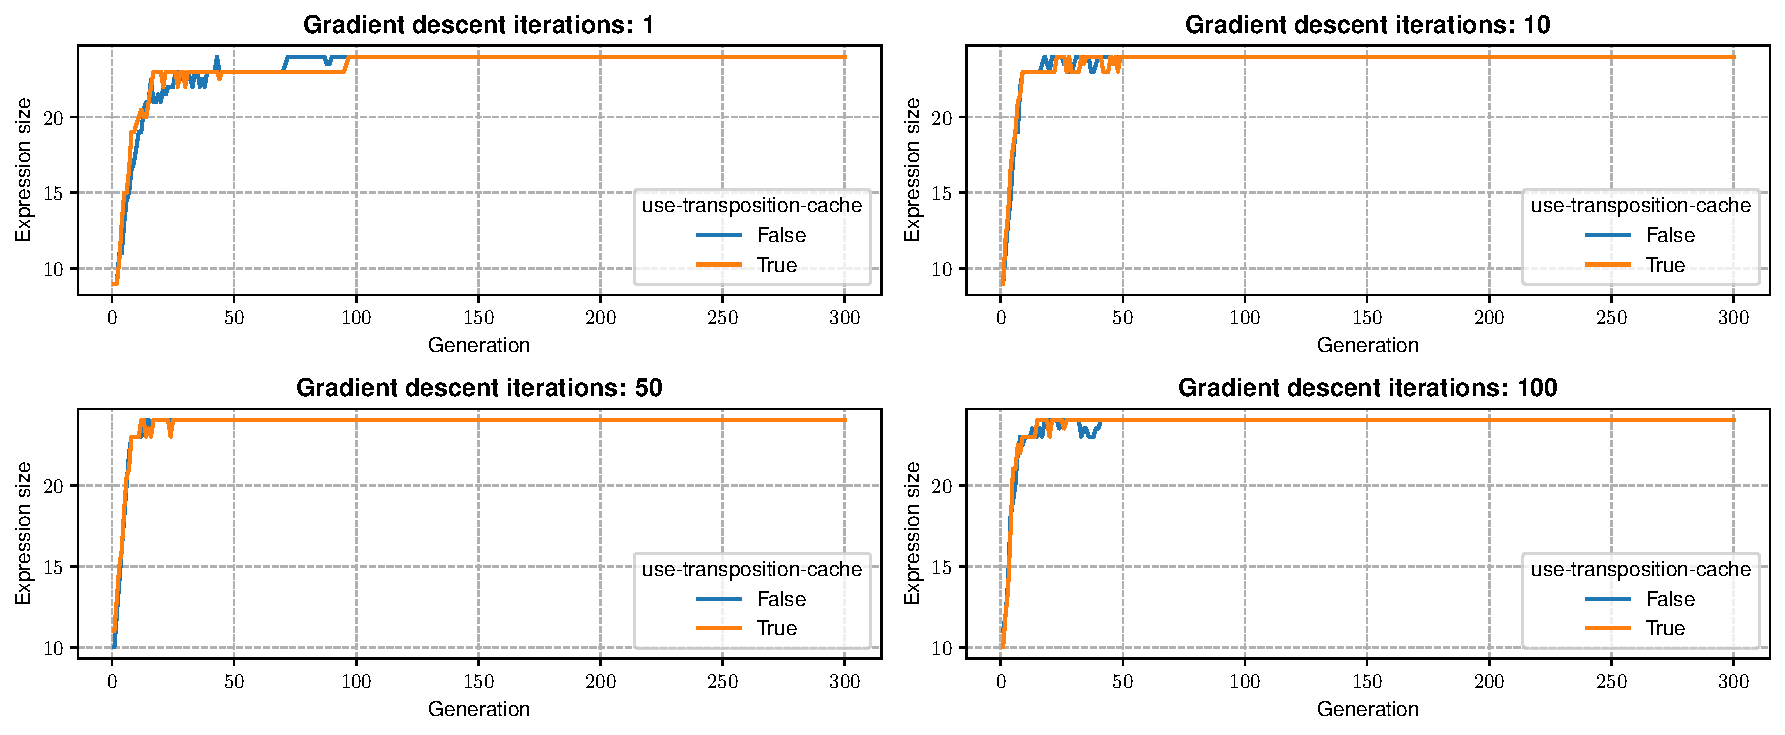
\includegraphics[width=\textwidth]{./fig/Nasa Battery 1_10_expression_size.pdf}
        \caption{Nasa Battery 1\_10 Expression Size}
    \end{figure}
\end{frame}

\begin{frame}
    \frametitle{Preliminary Results}

    \begin{figure}
        \centering
        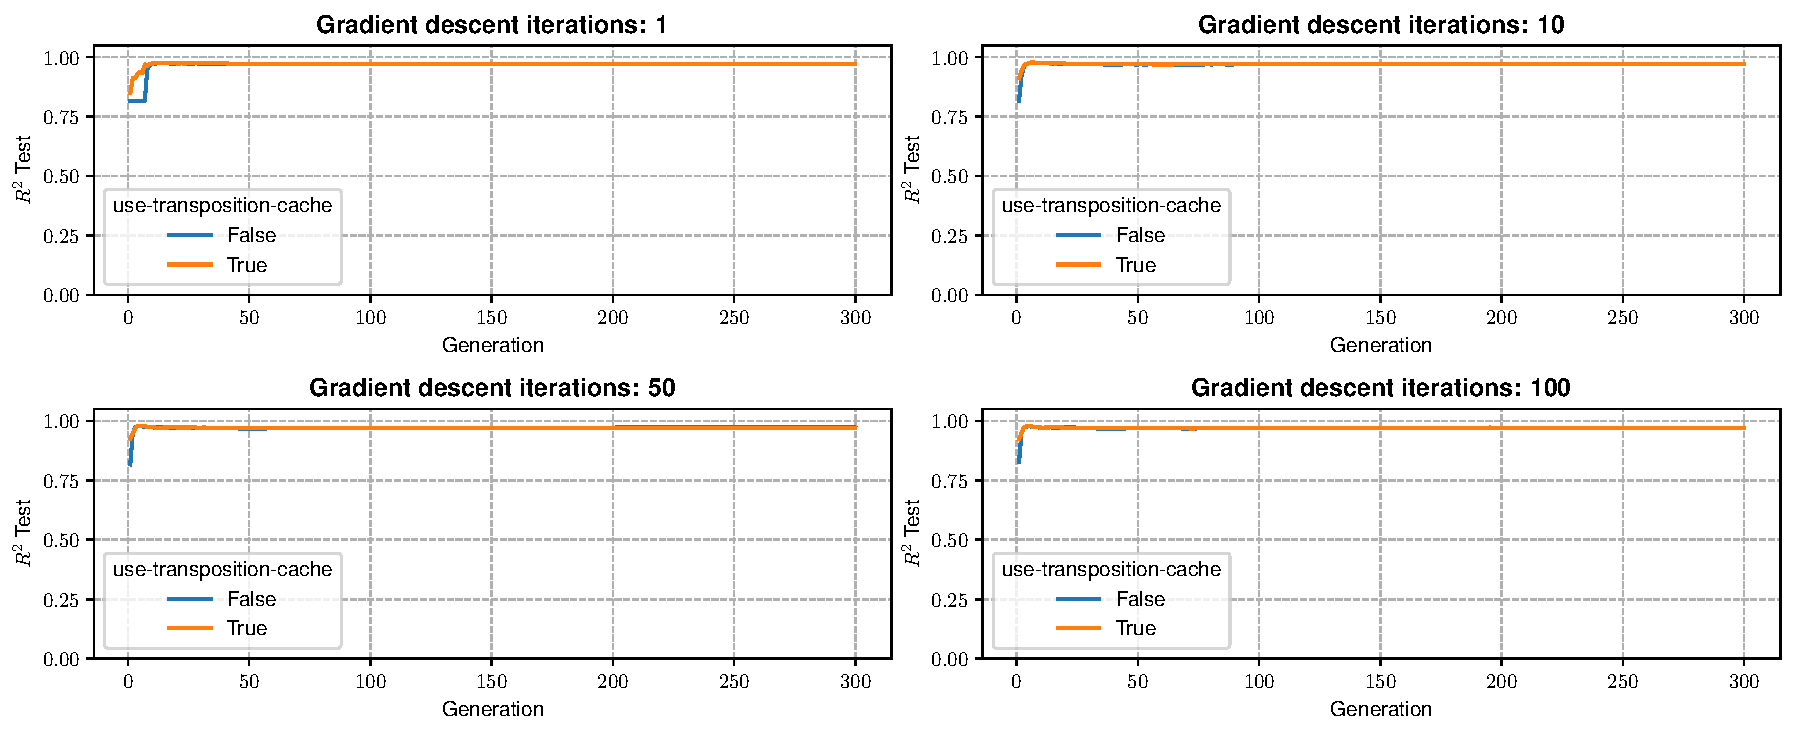
\includegraphics[width=\textwidth]{./fig/Nasa Battery 2_20_test_performance.pdf}
        \caption{Nasa Battery 2\_20 Test Performance}
    \end{figure}
\end{frame}

\begin{frame}
    \frametitle{Preliminary Results}

    \begin{figure}
        \centering
        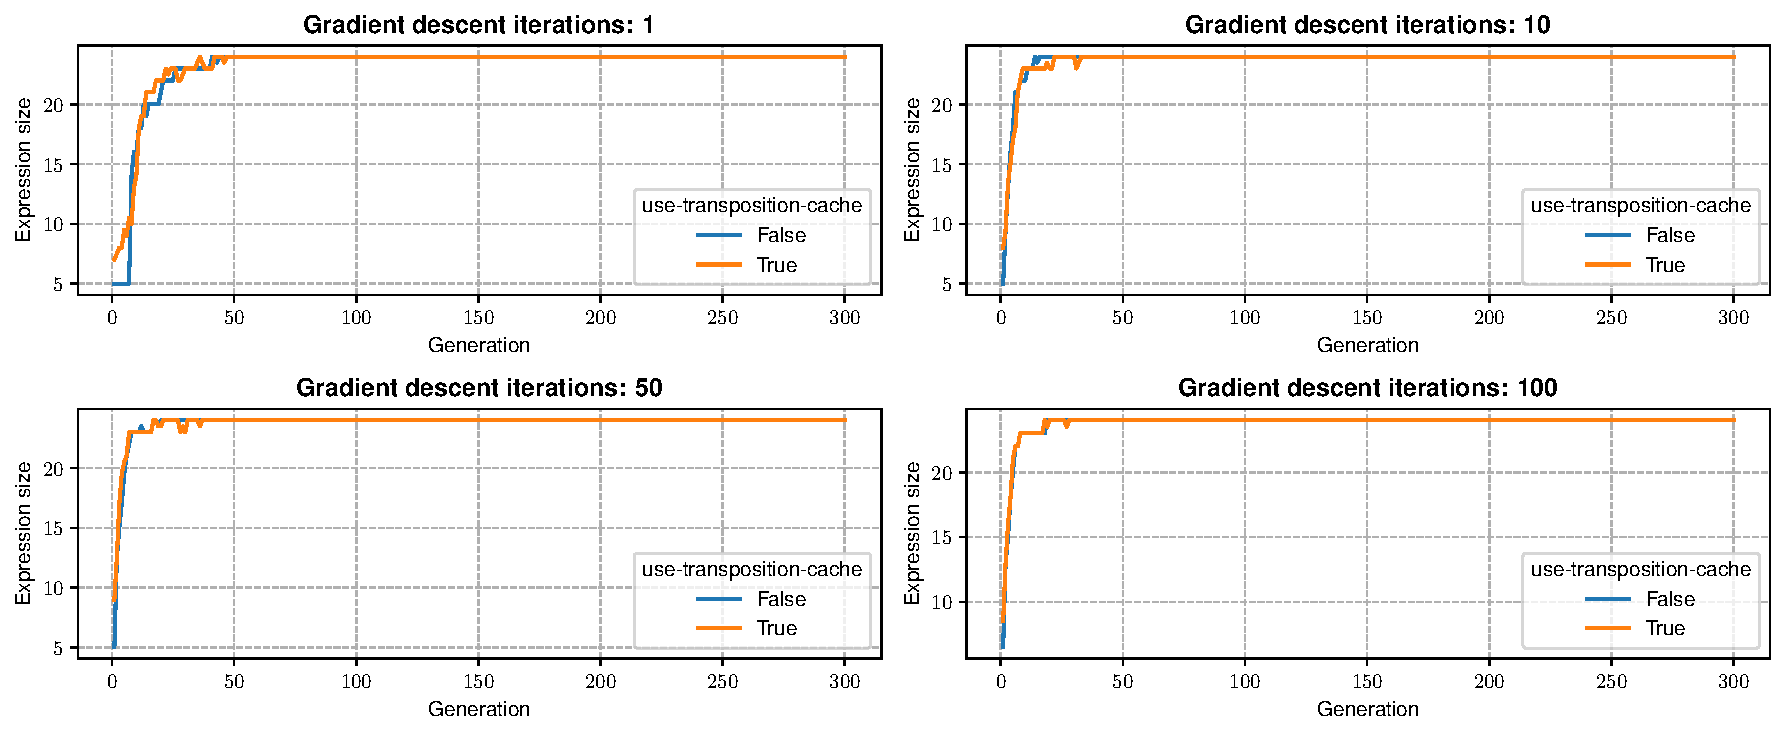
\includegraphics[width=\textwidth]{./fig/Nasa Battery 2_20_expression_size.pdf}
        \caption{Nasa Battery 2\_20 Expression Size}
    \end{figure}
\end{frame}

\begin{frame}
    \frametitle{Preliminary Results}

    \begin{figure}
        \centering
        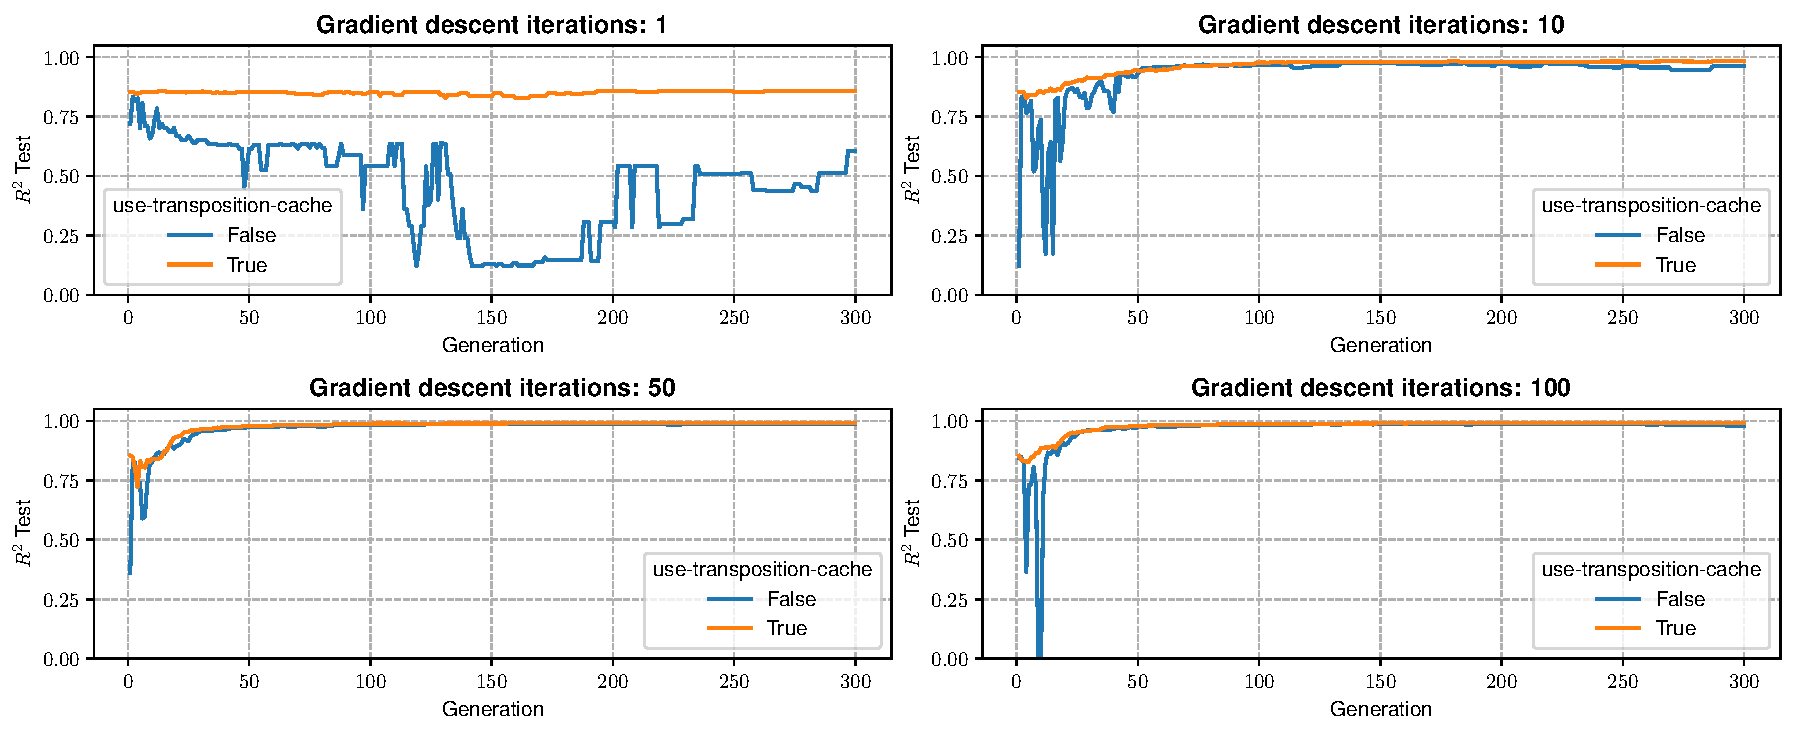
\includegraphics[width=\textwidth]{./fig/Nikuradse-I_test_performance.pdf}
        \caption{Nikuradse-I Test Performance}
    \end{figure}
\end{frame}

\begin{frame}
    \frametitle{Preliminary Results}

    \begin{figure}
        \centering
        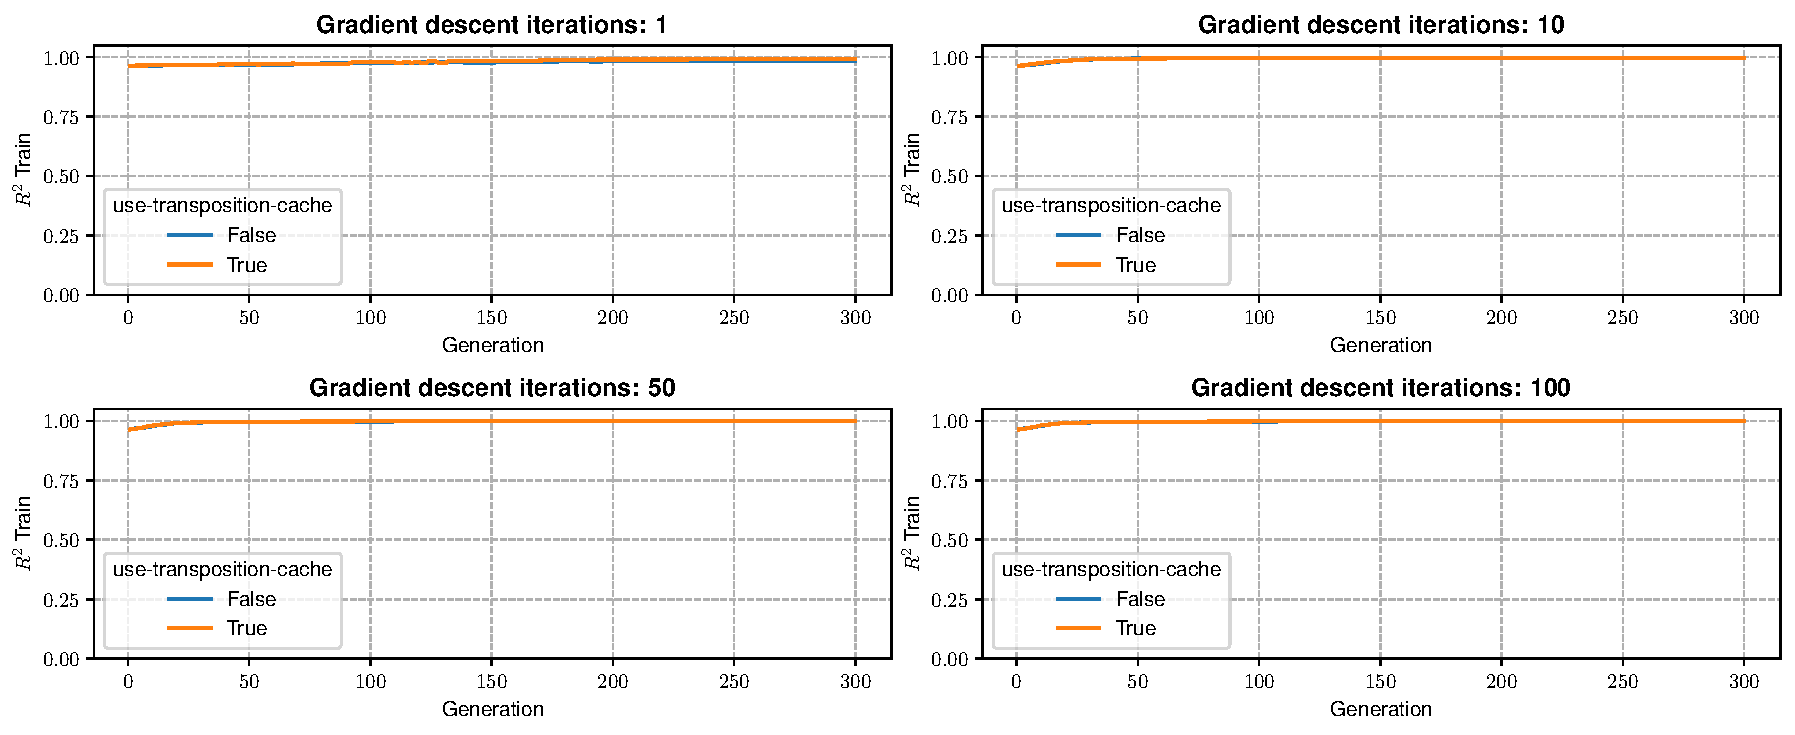
\includegraphics[width=\textwidth]{./fig/Nikuradse-I_train_performance.pdf}
        \caption{Nikuradse-I Train Performance}
    \end{figure}
\end{frame}

\begin{frame}
    \frametitle{Preliminary Results}

    \begin{figure}
        \centering
        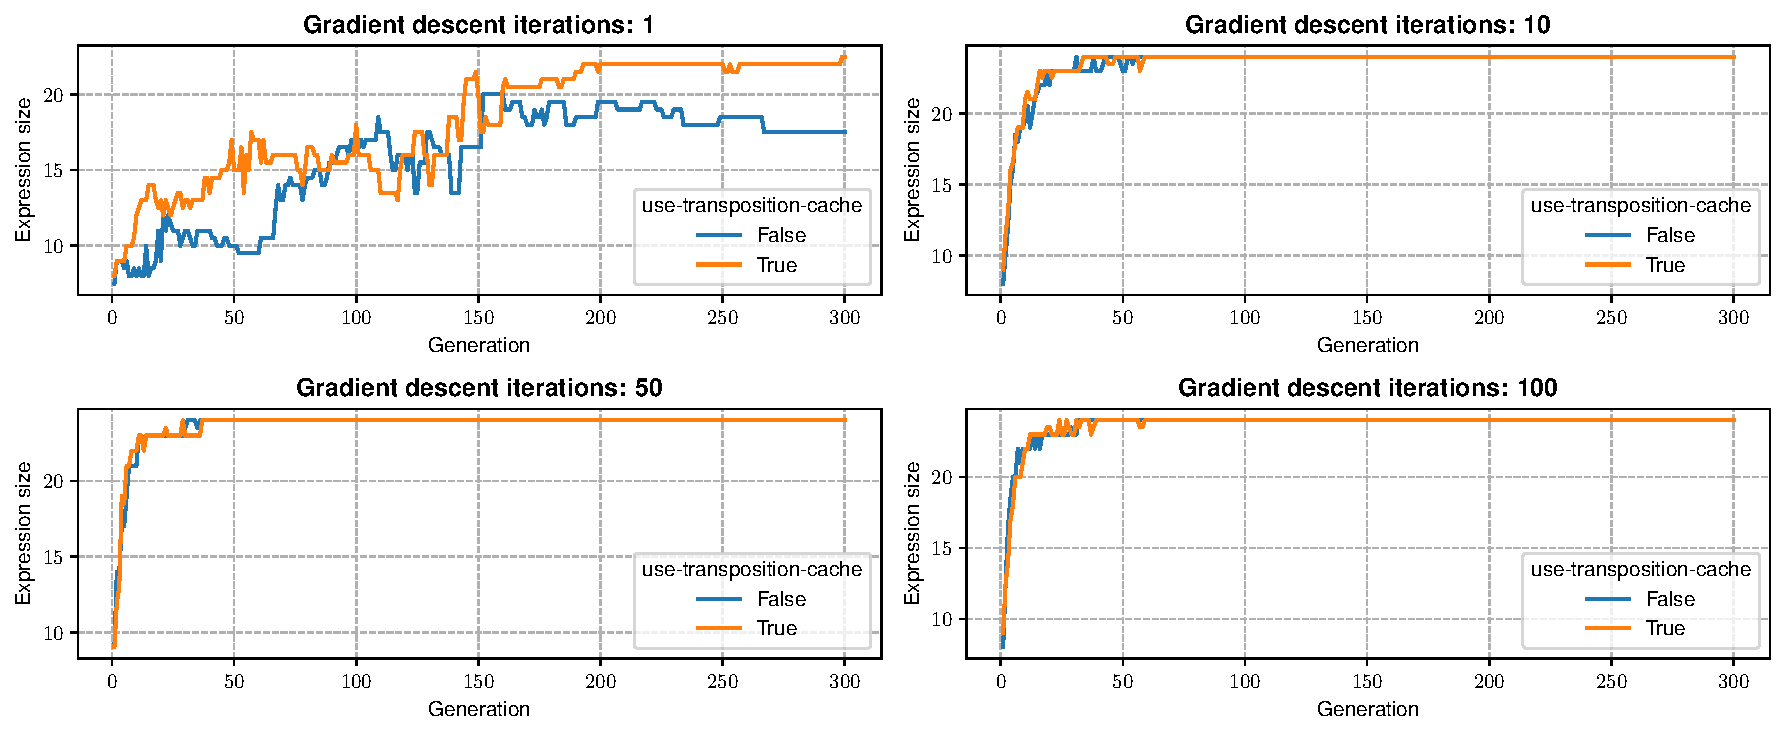
\includegraphics[width=\textwidth]{./fig/Nikuradse-I_expression_size.pdf}
        \caption{Nikuradse-I Expression Size}
    \end{figure}
\end{frame}

\begin{frame}
    \frametitle{Preliminary Results}

    \begin{figure}
        \centering
        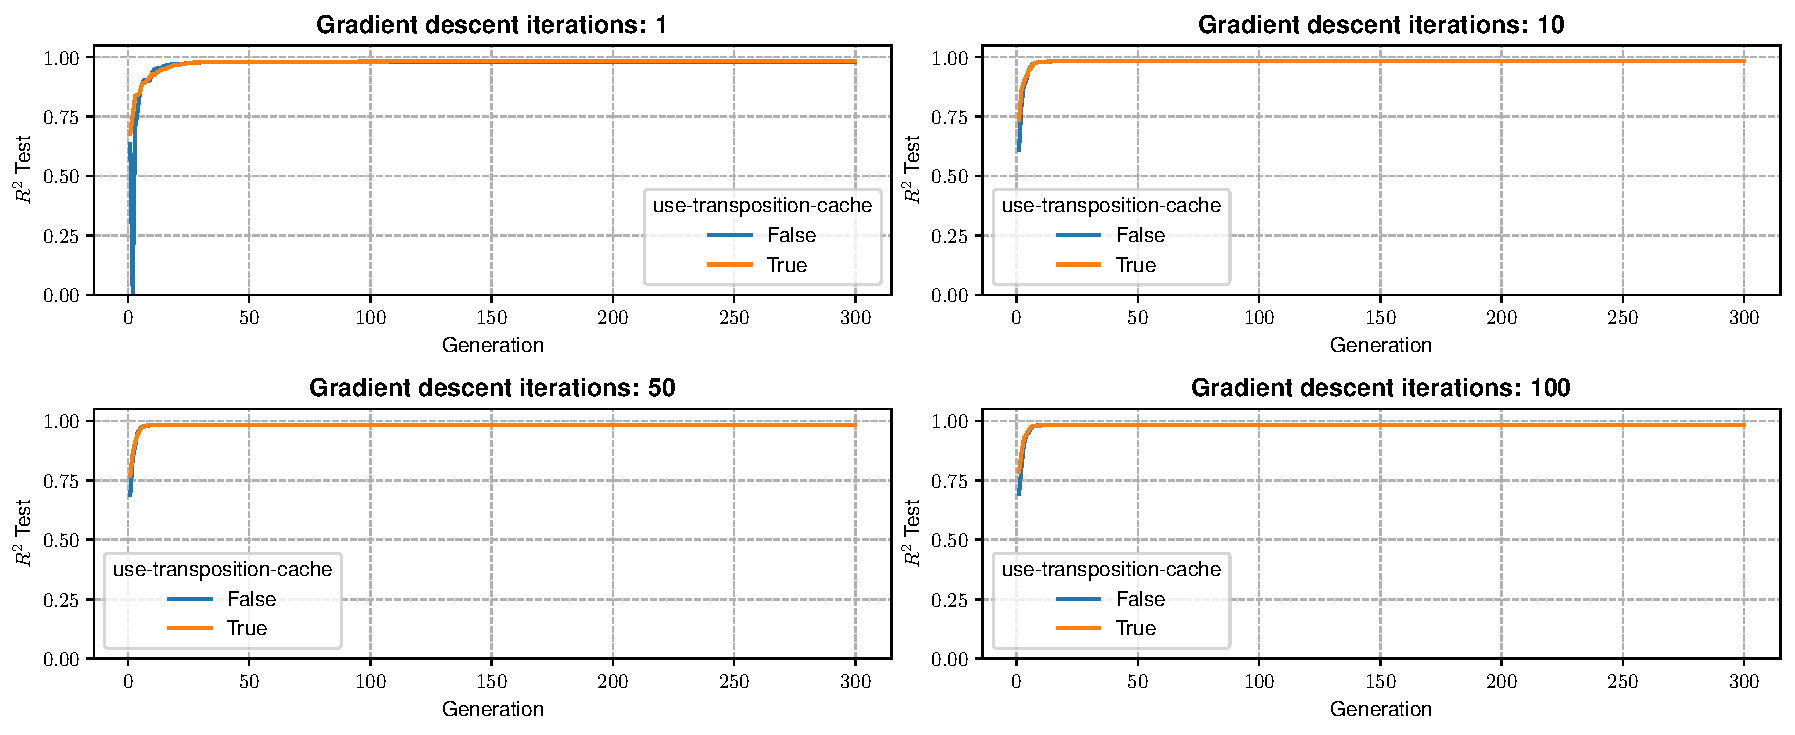
\includegraphics[width=\textwidth]{./fig/Nikuradse-II_test_performance.pdf}
        \caption{Nikuradse-II Test Performance}
    \end{figure}
\end{frame}

\begin{frame}
    \frametitle{Preliminary Results}

    \begin{figure}
        \centering
        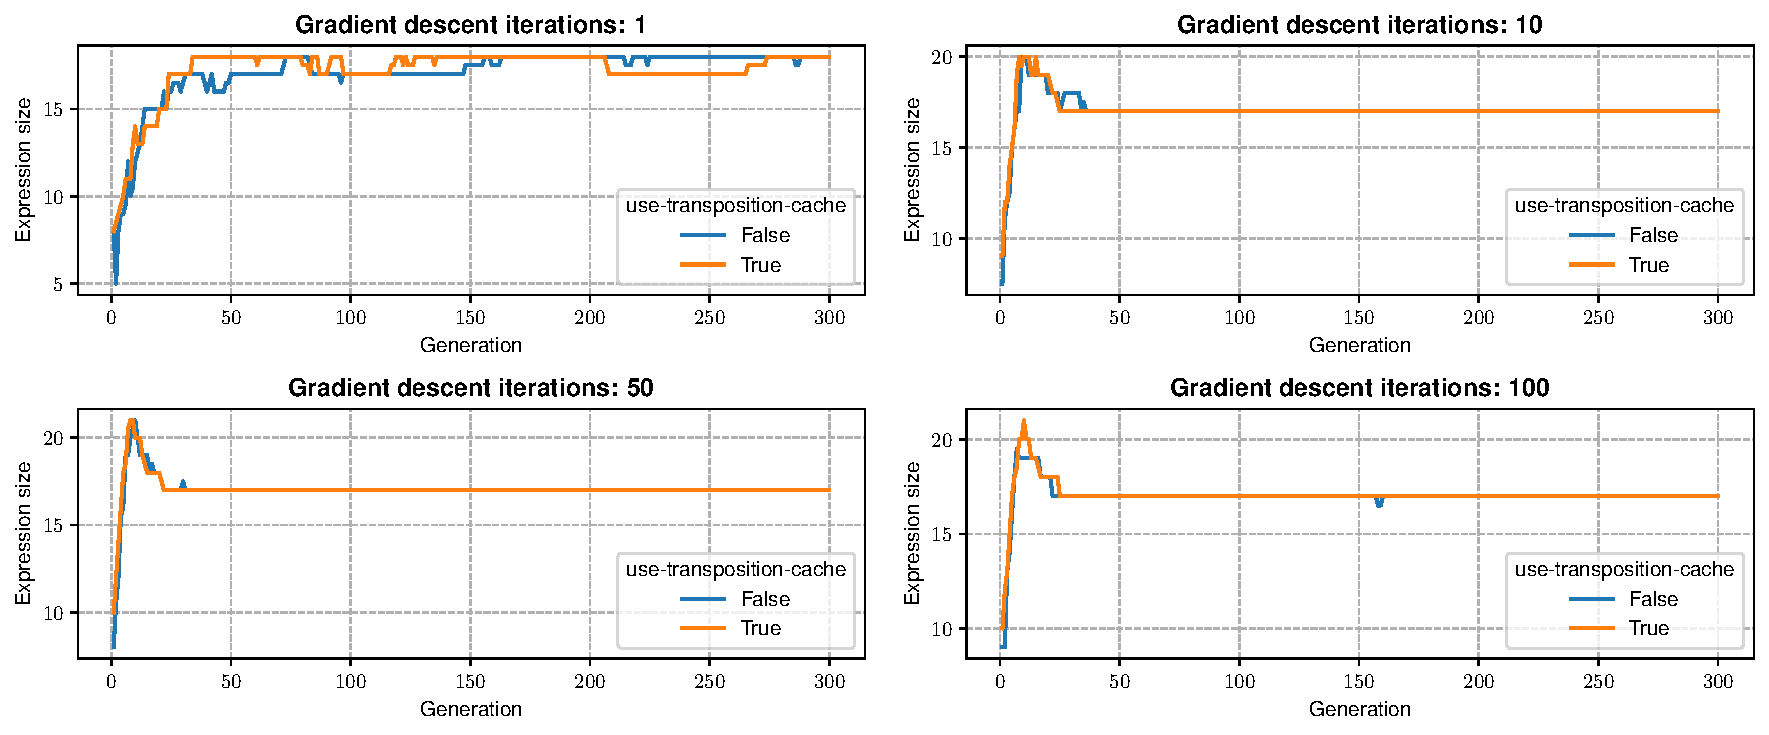
\includegraphics[width=\textwidth]{./fig/Nikuradse-II_expression_size.pdf}
        \caption{Nikuradse-II Expression Size}
    \end{figure}
\end{frame}

\begin{frame}
    \frametitle{Conclusions}

    \AB{Zobrist Hashing}

    \begin{itemize}
        \item Low overhead, easy to implement, resulting in speedups and energy savings
        \item \A{Fitness caching} may induce a more beneficial fitness landscape and prevent overfitting
        \item \A{Novelty promotion} not as reliable in improving performance
    \end{itemize}
    \bigskip

    \AB{Future Work}
    \begin{itemize}
        \item Deeper look at algorithm dynamics with caching
        \item Improved caching strategies: LRU cache, generational
        \item Better integration with search operators to promote novelty
        \item Attempt to capture symmetries and other equivalent sub-expressions
    \end{itemize}
\end{frame}

% \begin{frame}
%     \frametitle{Preliminary Results}

%     \begin{description}
%         \item[TC] Transposition cache (fitness)
%         \item[TO] Transposition operators (novelty)
%     \end{description}

%     \begin{table}
%         Flow Stress, 1 gradient descent iteration\\ median test performance ($R^2$ test $\pm$ std. dev.)
%         \medskip

%         \begin{tblr}{l|rrl}
%                    & TO=ON & TO=OFF\\
%             \hline
%             TC=ON  & 0.942 $\pm$ 0.555 & 0.942 $\pm$ 0.028\\
%             TC=OFF & 0.911 $\pm$ 23.920 & 0.911 $\pm$ 0.020\\
%         \end{tblr}
%     \end{table}
% \end{frame}

% \begin{frame}
%     \frametitle{Preliminary Results}

%     \begin{figure}
%         \centering
%         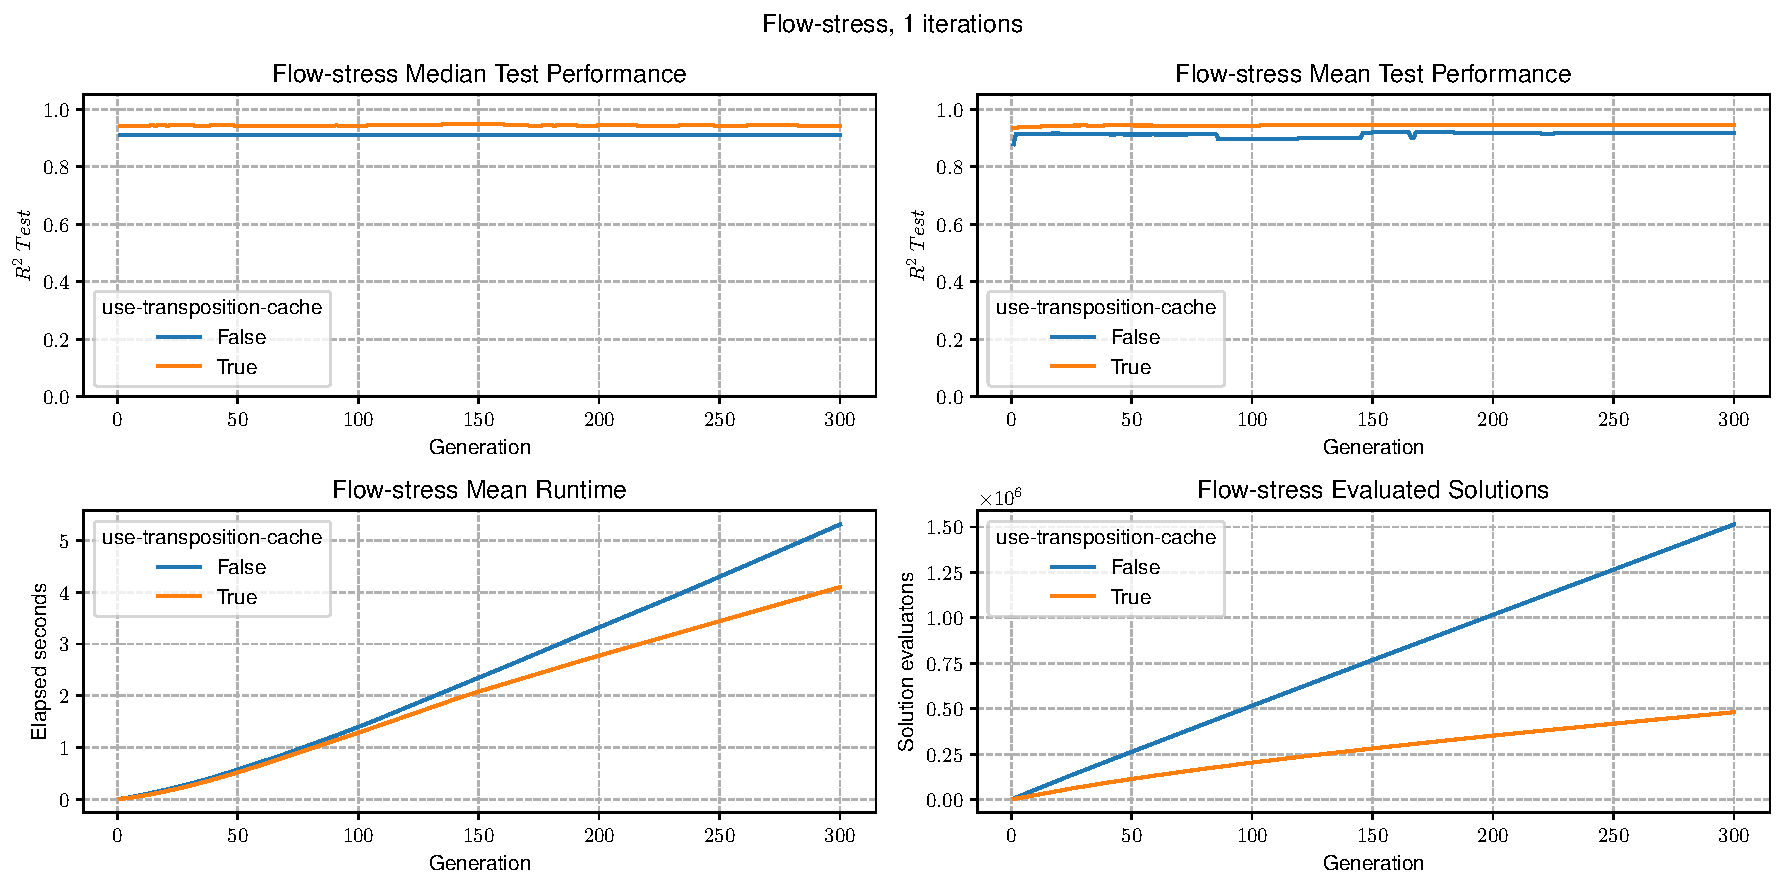
\includegraphics[width=0.88\textwidth]{./fig/Flow-stress_1_cache_only.pdf}
%         \caption{Flow Stress, 1 gradient descent iteration}
%     \end{figure}
% \end{frame}

% \begin{frame}
%     \frametitle{Preliminary Results}

%     \begin{figure}
%         \centering
%         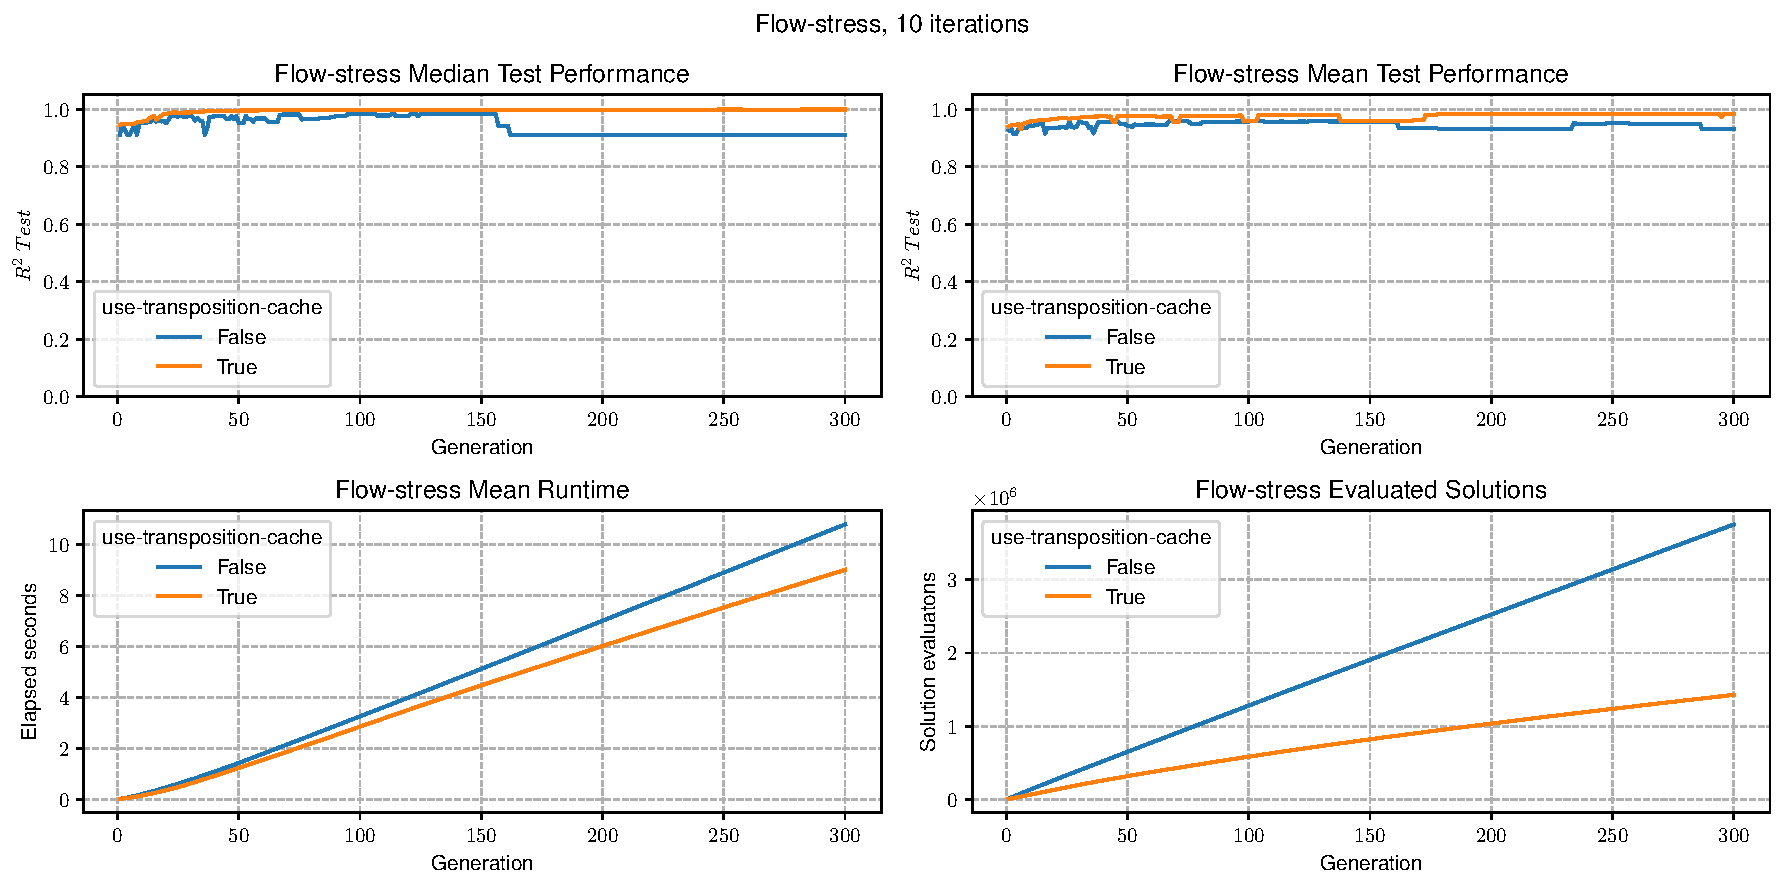
\includegraphics[width=0.88\textwidth]{./fig/Flow-stress_10_cache_only.pdf}
%         \caption{Flow Stress, 10 gradient descent iterations}
%     \end{figure}
% \end{frame}

% \begin{frame}
%     \frametitle{Preliminary Results}

%     \begin{figure}
%         \centering
%         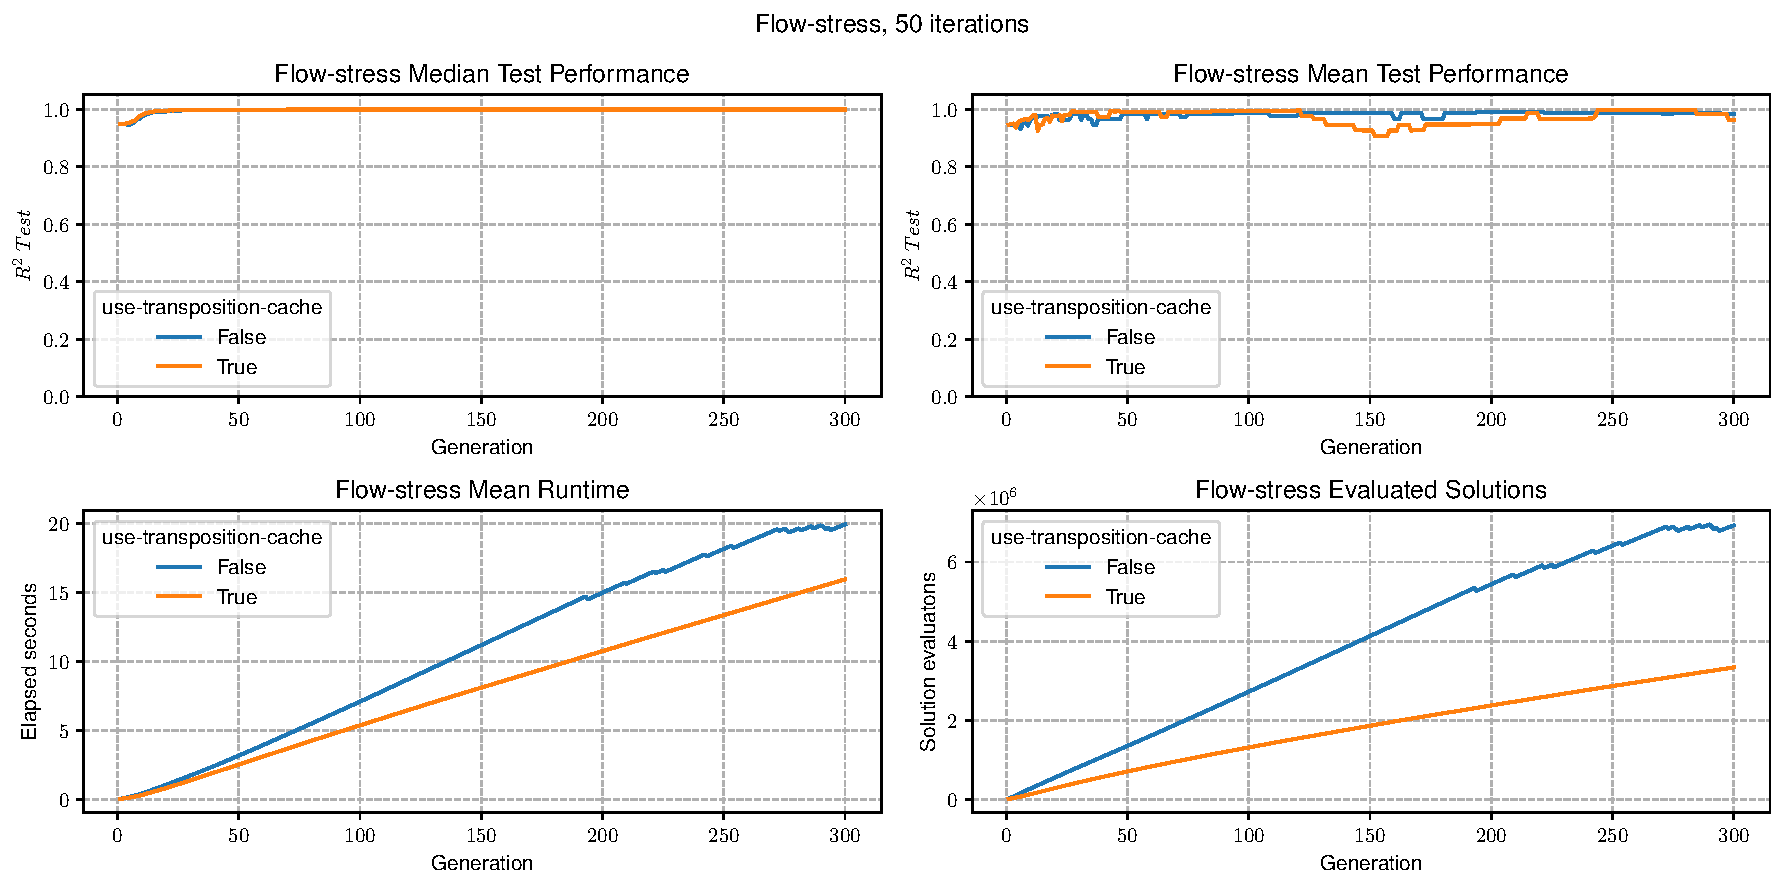
\includegraphics[width=0.88\textwidth]{./fig/Flow-stress_50_cache_only.pdf}
%         \caption{Flow Stress, 50 gradient descent iterations}
%     \end{figure}
% \end{frame}

% \begin{frame}
%     \frametitle{Preliminary Results}

%     \begin{figure}
%         \centering
%         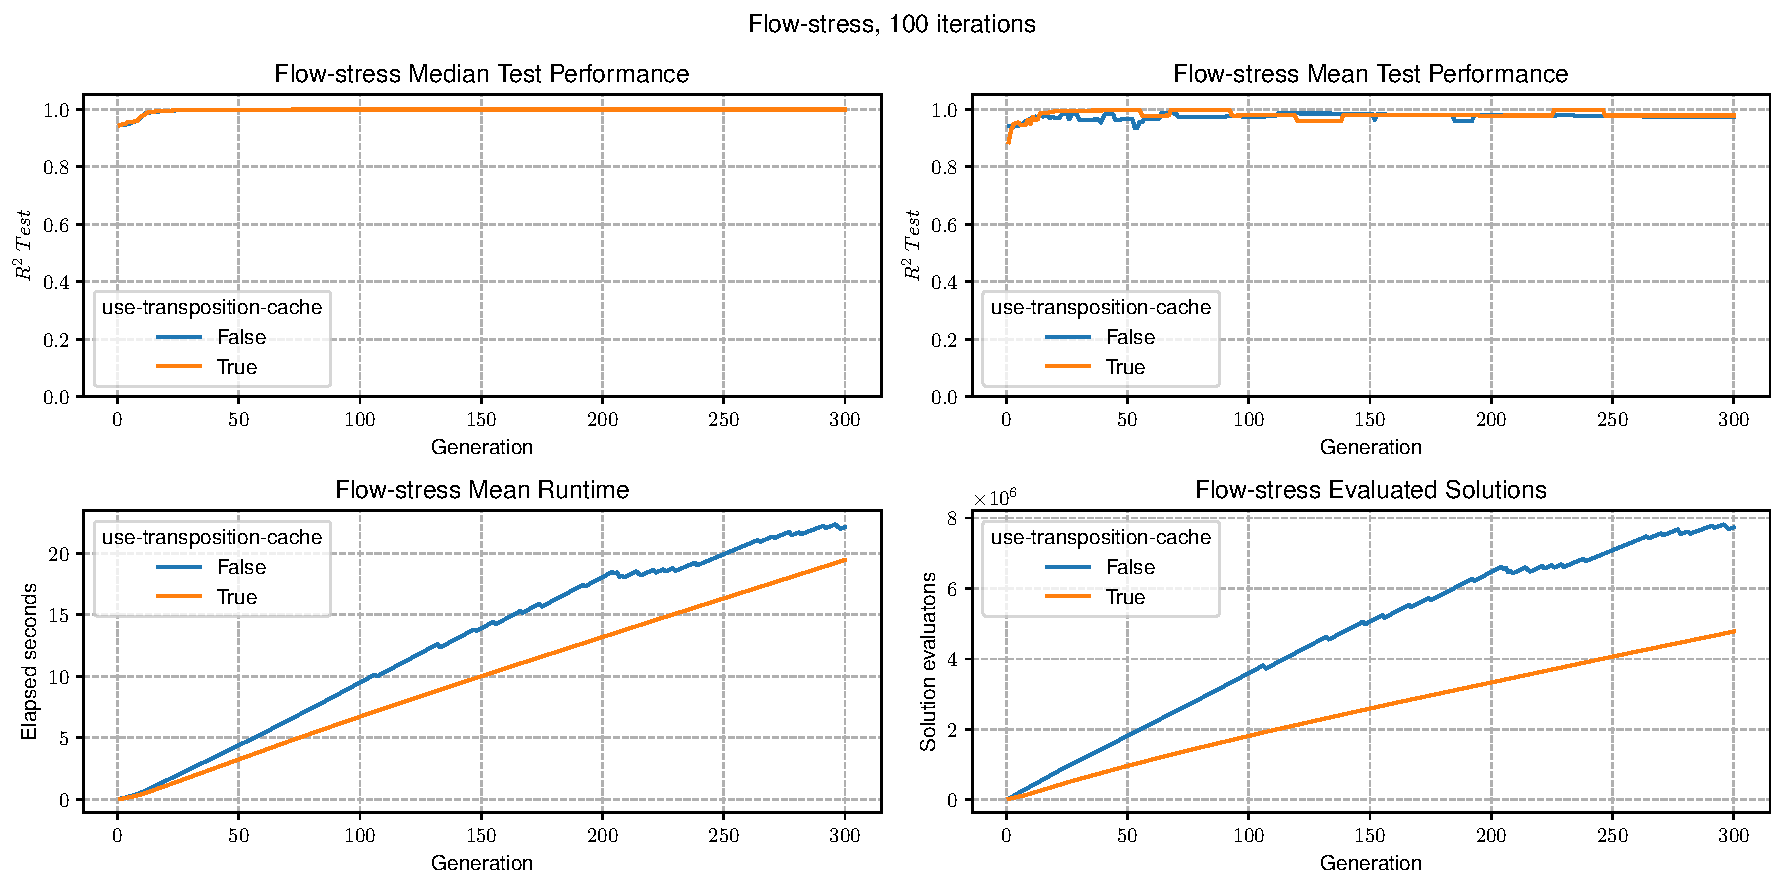
\includegraphics[width=0.88\textwidth]{./fig/Flow-stress_100_cache_only.pdf}
%         \caption{Flow Stress, 100 gradient descent iterations}
%     \end{figure}
% \end{frame}
\end{document}